\documentclass{article}

% Needs to be loaded before cleveref, so we can specify the name
% of a `listing` environment (https://tex.stackexchange.com/a/47694)
\usepackage{listings}
%%% Local Variables:
%%% mode: latex
%%% TeX-master: "../main"
%%% End:

% Recommended, but optional, packages for figures and better typesetting:
\usepackage{microtype}
\usepackage{graphicx}
\usepackage{booktabs} % for professional tables

% hyperref makes hyperlinks in the resulting PDF.
% If your build breaks (sometimes temporarily if a hyperlink spans a page)
% please comment out the following usepackage line and replace
% \usepackage{icml2024} with \usepackage[nohyperref]{icml2024} above.
\usepackage{hyperref} % hyperlinks

% Attempt to make hyperref and algorithmic work together better:
\newcommand{\theHalgorithm}{\arabic{algorithm}}

% Use the following line for the initial blind version submitted for review:
% \usepackage{icml2024}

% If accepted, instead use the following line for the camera-ready submission:
\usepackage[accepted]{icml2024}

% For theorems and such
\usepackage{amsmath}
\usepackage{amssymb}
\usepackage{mathtools}
\usepackage{amsthm}

% if you use cleveref..
\usepackage[capitalize,noabbrev]{cleveref}

%%%%%%%%%%%%%%%%%%%%%%%%%%%%%%%%
% THEOREMS
%%%%%%%%%%%%%%%%%%%%%%%%%%%%%%%%
\theoremstyle{plain}
\newtheorem{theorem}{Theorem}[section]
\newtheorem{proposition}[theorem]{Proposition}
\newtheorem{lemma}[theorem]{Lemma}
\newtheorem{corollary}[theorem]{Corollary}
\theoremstyle{definition}
\newtheorem{definition}[theorem]{Definition}
\newtheorem{assumption}[theorem]{Assumption}
\newtheorem{example}[theorem]{Example}
\theoremstyle{remark}
\newtheorem{remark}[theorem]{Remark}
%%% Local Variables:
%%% mode: latex
%%% TeX-master: "../main"
%%% End:

% requirements
\usepackage{amsmath}
\usepackage{amssymb}
\usepackage{bm}
\usepackage{mathtools}

% Random variables
\def\reta{{\textnormal{$\eta$}}}
\def\ra{{\textnormal{a}}}
\def\rb{{\textnormal{b}}}
\def\rc{{\textnormal{c}}}
\def\rd{{\textnormal{d}}}
\def\re{{\textnormal{e}}}
\def\rf{{\textnormal{f}}}
\def\rg{{\textnormal{g}}}
\def\rh{{\textnormal{h}}}
\def\ri{{\textnormal{i}}}
\def\rj{{\textnormal{j}}}
\def\rk{{\textnormal{k}}}
\def\rl{{\textnormal{l}}}
% rm is already a command, just don't name any random variables m
\def\rn{{\textnormal{n}}}
\def\ro{{\textnormal{o}}}
\def\rp{{\textnormal{p}}}
\def\rq{{\textnormal{q}}}
\def\rr{{\textnormal{r}}}
\def\rs{{\textnormal{s}}}
\def\rt{{\textnormal{t}}}
\def\ru{{\textnormal{u}}}
\def\rv{{\textnormal{v}}}
\def\rw{{\textnormal{w}}}
\def\rx{{\textnormal{x}}}
\def\ry{{\textnormal{y}}}
\def\rz{{\textnormal{z}}}

% Random vectors
\def\rvepsilon{{\mathbf{\epsilon}}}
\def\rvtheta{{\mathbf{\theta}}}
\def\rva{{\mathbf{a}}}
\def\rvb{{\mathbf{b}}}
\def\rvc{{\mathbf{c}}}
\def\rvd{{\mathbf{d}}}
\def\rve{{\mathbf{e}}}
\def\rvf{{\mathbf{f}}}
\def\rvg{{\mathbf{g}}}
\def\rvh{{\mathbf{h}}}
\def\rvu{{\mathbf{i}}}
\def\rvj{{\mathbf{j}}}
\def\rvk{{\mathbf{k}}}
\def\rvl{{\mathbf{l}}}
\def\rvm{{\mathbf{m}}}
\def\rvn{{\mathbf{n}}}
\def\rvo{{\mathbf{o}}}
\def\rvp{{\mathbf{p}}}
\def\rvq{{\mathbf{q}}}
\def\rvr{{\mathbf{r}}}
\def\rvs{{\mathbf{s}}}
\def\rvt{{\mathbf{t}}}
\def\rvu{{\mathbf{u}}}
\def\rvv{{\mathbf{v}}}
\def\rvw{{\mathbf{w}}}
\def\rvx{{\mathbf{x}}}
\def\rvy{{\mathbf{y}}}
\def\rvz{{\mathbf{z}}}

% Elements of random vectors
\def\erva{{\textnormal{a}}}
\def\ervb{{\textnormal{b}}}
\def\ervc{{\textnormal{c}}}
\def\ervd{{\textnormal{d}}}
\def\erve{{\textnormal{e}}}
\def\ervf{{\textnormal{f}}}
\def\ervg{{\textnormal{g}}}
\def\ervh{{\textnormal{h}}}
\def\ervi{{\textnormal{i}}}
\def\ervj{{\textnormal{j}}}
\def\ervk{{\textnormal{k}}}
\def\ervl{{\textnormal{l}}}
\def\ervm{{\textnormal{m}}}
\def\ervn{{\textnormal{n}}}
\def\ervo{{\textnormal{o}}}
\def\ervp{{\textnormal{p}}}
\def\ervq{{\textnormal{q}}}
\def\ervr{{\textnormal{r}}}
\def\ervs{{\textnormal{s}}}
\def\ervt{{\textnormal{t}}}
\def\ervu{{\textnormal{u}}}
\def\ervv{{\textnormal{v}}}
\def\ervw{{\textnormal{w}}}
\def\ervx{{\textnormal{x}}}
\def\ervy{{\textnormal{y}}}
\def\ervz{{\textnormal{z}}}

% Random matrices
\def\rmA{{\mathbf{A}}}
\def\rmB{{\mathbf{B}}}
\def\rmC{{\mathbf{C}}}
\def\rmD{{\mathbf{D}}}
\def\rmE{{\mathbf{E}}}
\def\rmF{{\mathbf{F}}}
\def\rmG{{\mathbf{G}}}
\def\rmH{{\mathbf{H}}}
\def\rmI{{\mathbf{I}}}
\def\rmJ{{\mathbf{J}}}
\def\rmK{{\mathbf{K}}}
\def\rmL{{\mathbf{L}}}
\def\rmM{{\mathbf{M}}}
\def\rmN{{\mathbf{N}}}
\def\rmO{{\mathbf{O}}}
\def\rmP{{\mathbf{P}}}
\def\rmQ{{\mathbf{Q}}}
\def\rmR{{\mathbf{R}}}
\def\rmS{{\mathbf{S}}}
\def\rmT{{\mathbf{T}}}
\def\rmU{{\mathbf{U}}}
\def\rmV{{\mathbf{V}}}
\def\rmW{{\mathbf{W}}}
\def\rmX{{\mathbf{X}}}
\def\rmY{{\mathbf{Y}}}
\def\rmZ{{\mathbf{Z}}}

% Elements of random matrices
\def\ermA{{\textnormal{A}}}
\def\ermB{{\textnormal{B}}}
\def\ermC{{\textnormal{C}}}
\def\ermD{{\textnormal{D}}}
\def\ermE{{\textnormal{E}}}
\def\ermF{{\textnormal{F}}}
\def\ermG{{\textnormal{G}}}
\def\ermH{{\textnormal{H}}}
\def\ermI{{\textnormal{I}}}
\def\ermJ{{\textnormal{J}}}
\def\ermK{{\textnormal{K}}}
\def\ermL{{\textnormal{L}}}
\def\ermM{{\textnormal{M}}}
\def\ermN{{\textnormal{N}}}
\def\ermO{{\textnormal{O}}}
\def\ermP{{\textnormal{P}}}
\def\ermQ{{\textnormal{Q}}}
\def\ermR{{\textnormal{R}}}
\def\ermS{{\textnormal{S}}}
\def\ermT{{\textnormal{T}}}
\def\ermU{{\textnormal{U}}}
\def\ermV{{\textnormal{V}}}
\def\ermW{{\textnormal{W}}}
\def\ermX{{\textnormal{X}}}
\def\ermY{{\textnormal{Y}}}
\def\ermZ{{\textnormal{Z}}}

% Vectors
\def\vzero{{\bm{0}}}
\def\vone{{\bm{1}}}
\def\valpha{{\bm{\alpha}}}
\def\vbeta{{\bm{\beta}}}
\def\vmu{{\bm{\mu}}}
\def\vnu{{\bm{\nu}}}
\def\vtheta{{\bm{\theta}}}
\def\vepsilon{{\bm{\epsilon}}}
\def\vgamma{{\bm{\gamma}}}
\def\vdelta{{\bm{\delta}}}
\def\vDelta{{\bm{\Delta}}}
\def\va{{\bm{a}}}
\def\vb{{\bm{b}}}
\def\vc{{\bm{c}}}
\def\vd{{\bm{d}}}
\def\ve{{\bm{e}}}
\def\vetilde{\bm{\tilde{e}}}
\def\vell{{\bm{\ell}}}
\def\vf{{\bm{f}}}
\def\vg{{\bm{g}}}
\def\vh{{\bm{h}}}
\def\vi{{\bm{i}}}
\def\vj{{\bm{j}}}
\def\vk{{\bm{k}}}
\def\vl{{\bm{l}}}
\def\vm{{\bm{m}}}
\def\vmhat{{\bm{\hat{m}}}}
\def\vn{{\bm{n}}}
\def\vo{{\bm{o}}}
\def\vp{{\bm{p}}}
\def\vphi{{\bm{\phi}}}
\def\vpsi{{\bm{\psi}}}
\def\vq{{\bm{q}}}
\def\vr{{\bm{r}}}
\def\vs{{\bm{s}}}
\def\vstilde{\bm{\tilde{s}}}
\def\vsigma{{\bm{\sigma}}}
\def\vt{{\bm{t}}}
\def\vu{{\bm{u}}}
\def\vv{{\bm{v}}}
\def\vvhat{{\bm{\hat{v}}}}
\def\vw{{\bm{w}}}
\def\vx{{\bm{x}}}
\def\vy{{\bm{y}}}
\def\vytilde{{\bm{\tilde{y}}}}
\def\vyhat{{\bm{\hat{y}}}}
\def\vz{{\bm{z}}}

% Elements of vectors
\def\evalpha{{\alpha}}
\def\evbeta{{\beta}}
\def\evepsilon{{\epsilon}}
\def\evlambda{{\lambda}}
\def\evomega{{\omega}}
\def\evmu{{\mu}}
\def\evpsi{{\psi}}
\def\evsigma{{\sigma}}
\def\evtheta{{\theta}}
\def\eva{{a}}
\def\evb{{b}}
\def\evc{{c}}
\def\evd{{d}}
\def\eve{{e}}
\def\evf{{f}}
\def\evg{{g}}
\def\evh{{h}}
\def\evi{{i}}
\def\evj{{j}}
\def\evk{{k}}
\def\evl{{l}}
\def\evm{{m}}
\def\evn{{n}}
\def\evo{{o}}
\def\evp{{p}}
\def\evq{{q}}
\def\evr{{r}}
\def\evs{{s}}
\def\evt{{t}}
\def\evu{{u}}
\def\evv{{v}}
\def\evw{{w}}
\def\evx{{x}}
\def\evy{{y}}
\def\evyhat{{\hat{y}}}
\def\evz{{z}}

% Matrix
\def\mA{{\bm{A}}}
\def\mB{{\bm{B}}}
\def\mC{{\bm{C}}}
\def\mD{{\bm{D}}}
\def\mE{{\bm{E}}}
\def\mF{{\bm{F}}}
\def\mG{{\bm{G}}}
\def\mGtilde{\bm{\tilde{G}}}
\def\mH{{\bm{H}}}
\def\mI{{\bm{I}}}
\def\mJ{{\bm{J}}}
\def\mK{{\bm{K}}}
\def\mL{{\bm{L}}}
\def\mM{{\bm{M}}}
\def\mN{{\bm{N}}}
\def\mO{{\bm{O}}}
\def\mP{{\bm{P}}}
\def\mQ{{\bm{Q}}}
\def\mR{{\bm{R}}}
\def\mS{{\bm{S}}}
\def\mT{{\bm{T}}}
\def\mU{{\bm{U}}}
\def\mV{{\bm{V}}}
\def\mW{{\bm{W}}}
\def\mX{{\bm{X}}}
\def\mY{{\bm{Y}}}
\def\mZ{{\bm{Z}}}
\def\mBeta{{\bm{\beta}}}
\def\mPhi{{\bm{\Phi}}}
\def\mPi{{\bm{\Pi}}}
\def\mLambda{{\bm{\Lambda}}}
\def\mSigma{{\bm{\Sigma}}}
\def\mStilde{\bm{\tilde{\mS}}}
\def\mGtilde{\bm{\tilde{\mG}}}
\def\mGoverline{{\bm{\overline{G}}}}

% Tensor
\DeclareMathAlphabet{\mathsfit}{\encodingdefault}{\sfdefault}{m}{sl}
\SetMathAlphabet{\mathsfit}{bold}{\encodingdefault}{\sfdefault}{bx}{n}
\newcommand{\tens}[1]{\bm{\mathsfit{#1}}}
\def\tA{{\tens{A}}}
\def\tB{{\tens{B}}}
\def\tC{{\tens{C}}}
\def\tD{{\tens{D}}}
\def\tE{{\tens{E}}}
\def\tF{{\tens{F}}}
\def\tG{{\tens{G}}}
\def\tH{{\tens{H}}}
\def\tI{{\tens{I}}}
\def\tJ{{\tens{J}}}
\def\tK{{\tens{K}}}
\def\tL{{\tens{L}}}
\def\tM{{\tens{M}}}
\def\tN{{\tens{N}}}
\def\tO{{\tens{O}}}
\def\tP{{\tens{P}}}
\def\tPi{\bm{\mathsf{\Pi}}}
\def\tQ{{\tens{Q}}}
\def\tR{{\tens{R}}}
\def\tS{{\tens{S}}}
\def\tT{{\tens{T}}}
\def\tU{{\tens{U}}}
\def\tV{{\tens{V}}}
\def\tW{{\tens{W}}}
\def\tX{{\tens{X}}}
\def\tY{{\tens{Y}}}
\def\tZ{{\tens{Z}}}

% Graph
\def\gA{{\mathcal{A}}}
\def\gB{{\mathcal{B}}}
\def\gC{{\mathcal{C}}}
\def\gD{{\mathcal{D}}}
\def\gE{{\mathcal{E}}}
\def\gF{{\mathcal{F}}}
\def\gG{{\mathcal{G}}}
\def\gH{{\mathcal{H}}}
\def\gI{{\mathcal{I}}}
\def\gJ{{\mathcal{J}}}
\def\gK{{\mathcal{K}}}
\def\gL{{\mathcal{L}}}
\def\gM{{\mathcal{M}}}
\def\gN{{\mathcal{N}}}
\def\gO{{\mathcal{O}}}
\def\gP{{\mathcal{P}}}
\def\gQ{{\mathcal{Q}}}
\def\gR{{\mathcal{R}}}
\def\gS{{\mathcal{S}}}
\def\gT{{\mathcal{T}}}
\def\gU{{\mathcal{U}}}
\def\gV{{\mathcal{V}}}
\def\gW{{\mathcal{W}}}
\def\gX{{\mathcal{X}}}
\def\gY{{\mathcal{Y}}}
\def\gZ{{\mathcal{Z}}}

% Sets
\def\sA{{\mathbb{A}}}
\def\sB{{\mathbb{B}}}
\def\sC{{\mathbb{C}}}
\def\sD{{\mathbb{D}}}
% Don't use a set called E, because this would be the same as our symbol
% for expectation.
\def\sF{{\mathbb{F}}}
\def\sG{{\mathbb{G}}}
\def\sH{{\mathbb{H}}}
\def\sI{{\mathbb{I}}}
\def\sJ{{\mathbb{J}}}
\def\sK{{\mathbb{K}}}
\def\sL{{\mathbb{L}}}
\def\sM{{\mathbb{M}}}
\def\sN{{\mathbb{N}}}
\def\sO{{\mathbb{O}}}
\def\sP{{\mathbb{P}}}
\def\sQ{{\mathbb{Q}}}
\def\sR{{\mathbb{R}}}
\def\sS{{\mathbb{S}}}
\def\sT{{\mathbb{T}}}
\def\sU{{\mathbb{U}}}
\def\sV{{\mathbb{V}}}
\def\sW{{\mathbb{W}}}
\def\sX{{\mathbb{X}}}
\def\sY{{\mathbb{Y}}}
\def\sYhat{{\hat{\mathbb{Y}}}}
\def\sZ{{\mathbb{Z}}}
% Blackboard Greek characters: https://tex.stackexchange.com/a/3260
\DeclareSymbolFont{bbold}{U}{bbold}{m}{n}
\DeclareSymbolFontAlphabet{\mathbbold}{bbold}
\def\sTheta{{\mathbbold{\Theta}}}
\def\sOmega{{\mathbbold{\Omega}}}

% Entries of a matrix
\def\emLambda{{\Lambda}}
\def\emA{{A}}
\def\emB{{B}}
\def\emC{{C}}
\def\emD{{D}}
\def\emE{{E}}
\def\emF{{F}}
\def\emG{{G}}
\def\emH{{H}}
\def\emI{{I}}
\def\emJ{{J}}
\def\emK{{K}}
\def\emL{{L}}
\def\emM{{M}}
\def\emN{{N}}
\def\emO{{O}}
\def\emP{{P}}
\def\emQ{{Q}}
\def\emR{{R}}
\def\emS{{S}}
\def\emT{{T}}
\def\emU{{U}}
\def\emV{{V}}
\def\emW{{W}}
\def\emX{{X}}
\def\emY{{Y}}
\def\emZ{{Z}}
\def\emSigma{{\Sigma}}
\def\emPi{{\Pi}}

% entries of a tensor
% Same font as tensor, without \bm wrapper
\newcommand{\etens}[1]{\mathsfit{#1}}
\def\etLambda{{\etens{\Lambda}}}
\def\etA{{\etens{A}}}
\def\etB{{\etens{B}}}
\def\etC{{\etens{C}}}
\def\etD{{\etens{D}}}
\def\etE{{\etens{E}}}
\def\etF{{\etens{F}}}
\def\etG{{\etens{G}}}
\def\etH{{\etens{H}}}
\def\etI{{\etens{I}}}
\def\etJ{{\etens{J}}}
\def\etK{{\etens{K}}}
\def\etL{{\etens{L}}}
\def\etM{{\etens{M}}}
\def\etN{{\etens{N}}}
\def\etO{{\etens{O}}}
\def\etP{{\etens{P}}}
\def\etPi{\mathsf{\Pi}}
\def\etQ{{\etens{Q}}}
\def\etR{{\etens{R}}}
\def\etS{{\etens{S}}}
\def\etT{{\etens{T}}}
\def\etU{{\etens{U}}}
\def\etV{{\etens{V}}}
\def\etW{{\etens{W}}}
\def\etX{{\etens{X}}}
\def\etY{{\etens{Y}}}
\def\etZ{{\etens{Z}}}

% The true underlying data generating distribution
\newcommand{\pdata}{p_{\mathrm{data}}}
% The empirical distribution defined by the training set
\newcommand{\ptrain}{\hat{p}_{\mathrm{data}}}
\newcommand{\Ptrain}{\hat{P}_{\mathrm{data}}}
% The model distribution
\newcommand{\pmodel}{p_{\rm{model}}}
\newcommand{\Pmodel}{P_{\rm{model}}}
\newcommand{\ptildemodel}{\tilde{p}_{\rm{model}}}
% Stochastic autoencoder distributions
\newcommand{\pencode}{p_{\rm{encoder}}}
\newcommand{\pdecode}{p_{\rm{decoder}}}
\newcommand{\precons}{p_{\rm{reconstruct}}}

\newcommand{\laplace}{\mathrm{Laplace}} % Laplace distribution

\newcommand{\E}{\mathbb{E}}
\newcommand{\Ls}{\mathcal{L}}
\newcommand{\R}{\mathbb{R}}
\newcommand{\emp}{\tilde{p}}
\newcommand{\lr}{\alpha}
\newcommand{\reg}{\lambda}
\newcommand{\rect}{\mathrm{rectifier}}
\newcommand{\softmax}{\mathrm{softmax}}
\newcommand{\onehot}{\mathrm{onehot}}
\newcommand{\sigmoid}{\sigma}
\newcommand{\softplus}{\zeta}
\newcommand{\KL}{D_{\mathrm{KL}}}
\newcommand{\Var}{\mathrm{Var}}
\newcommand{\standarderror}{\mathrm{SE}}
\newcommand{\Cov}{\mathrm{Cov}}
% Wolfram Mathworld says $L^2$ is for function spaces and $\ell^2$ is for vectors
% But then they seem to use $L^2$ for vectors throughout the site, and so does
% wikipedia.
\newcommand{\normlzero}{L^0}
\newcommand{\normlone}{L^1}
\newcommand{\normltwo}{L^2}
\newcommand{\normlp}{L^p}
\newcommand{\normmax}{L^\infty}

\newcommand{\parents}{Pa} % See usage in notation.tex. Chosen to match Daphne's book.

\DeclareMathOperator*{\argmax}{arg\,max}
\DeclareMathOperator*{\argmin}{arg\,min}
\DeclareMathOperator*{\minimize}{minimize}
\DeclareMathOperator*{\maximize}{maximize}

\DeclareMathOperator{\sign}{sign}
\DeclareMathOperator{\mean}{mean}
\DeclareMathOperator{\vmap}{vmap}
\DeclareMathOperator{\reshape}{reshape}
% \DeclareMathOperator{\Tr}{Tr} % already defined when using the 'physics' package
\DeclareMathOperator{\diag}{diag}
\DeclareMathOperator{\eig}{eig}
\DeclareMathOperator{\rank}{rank} % already defined when using the 'physics' package
\DeclareMathOperator{\vecspan}{span}
\DeclareMathOperator{\overlap}{overlap}
\DeclareMathOperator{\Cat}{Cat}
\DeclareMathOperator{\flatten}{vec}

%%%%% NEW MATH DEFINITIONS %%%%%
\newcommand{\jac}{\mathrm{J}}
\newcommand{\hess}{\mathrm{H}}
\newcommand{\ggn}{\mathrm{G}}
\newcommand{\fisher}{\mathrm{F}}
\newcommand{\kfac}{\mathrm{KFAC}}
% \newcommand{\grad}[1]{\ensuremath{\nabla_{\!{#1}}}} % already defined when using the 'physics' package
\newcommand{\naturalgrad}[1]{\ensuremath{\tilde{\nabla}_{\!{#1}}}}
\newcommand{\gradsquared}[1]{\ensuremath{\nabla_{\!{#1}}^{2}}}
\newcommand{\batchnorm}{\mathrm{BN}}
\DeclareMathOperator{\GL}{GL}
\DeclareMathOperator{\sym}{sym}
\DeclareMathOperator{\lift}{lift}
\let\grad\relax % delete the existing `grad' command
\DeclareMathOperator{\grad}{grad}
\DeclareMathOperator{\orbit}{orbit}

\let\ab\allowbreak

%%% Local Variables:
%%% mode: latex
%%% TeX-master: "../main"
%%% End:

% ===================================================================
% WRITING
% ===================================================================
\usepackage{paracol}
\usepackage{blindtext}
\newcommand{\felix}[1]{\textcolor{red}{[\textbf{Felix:} #1]}}
\newcommand{\balint}[1]{\textcolor{orange}{Bálint: #1}}
\usepackage{xspace}
\newcommand*{\ie}{i.e.\@\xspace}
\newcommand*{\iid}{i.i.d.\@\xspace}
\newcommand*{\wrt}{w.r.t.\@\xspace}
\newcommand*{\eg}{e.g.\@\xspace}
\newcommand*{\Ie}{I.e.\@\xspace}
\newcommand*{\Eg}{E.g.\@\xspace}

% ===================================================================
% COLORS
% ===================================================================
% VECTOR PRIMARY COLORS
\definecolor{VectorBlack}{RGB}{34, 34, 34}
\definecolor{VectorGray}{RGB}{239, 238, 237}

% VECTOR SECONDARY COLORS
\definecolor{VectorBlue}{RGB}{59, 69, 227}
\definecolor{VectorPink}{RGB}{253, 8, 238}
\definecolor{VectorOrange}{RGB}{250, 173, 26}
\definecolor{VectorTeal}{RGB}{82, 199, 222}
\newcommand{\colored}[2][VectorBlue]{{\color{#1}#2}}

% ===================================================================
% REFERENCES
% ===================================================================
\hypersetup{%
  colorlinks,
  citecolor = VectorBlue,%
  linkcolor = VectorBlue,%
  urlcolor = VectorPink,%
}%
% tell cleveref how to name a listing environment
\crefname{listing}{snippet}{snippets}
% Rename Listing into Snippet
\renewcommand{\lstlistingname}{Snippet}

% ===================================================================
% CODE BLOCKS
% ===================================================================
% define style for listings using the Vector color scheme
\lstdefinestyle{vector_institute}{
  backgroundcolor=\color{VectorGray!50},
  commentstyle=\bfseries\color{VectorBlue},
  keywordstyle=\bfseries\color{VectorBlack},
  numberstyle=\tiny\color{VectorBlack!50},
  stringstyle=\bfseries\color{VectorBlue},
  basicstyle=\ttfamily\scriptsize,
  xleftmargin=3.2ex,
  breakatwhitespace=false,
  breaklines=true,
  captionpos=t,
  keepspaces=true,
  numbers=left,
  numbersep=7pt,
  showspaces=false,
  showstringspaces=false,
  showtabs=false,
  tabsize=2,
  escapebegin={\color{VectorBlue}},
  linewidth=\linewidth,
  mathescape=true,
}
% use the above style as default
\lstset{style=vector_institute}

\usepackage{caption}
% modify captions of code blocks
\captionsetup[lstlisting]{%
  font={scriptsize},%
  justification=raggedright,%
  singlelinecheck=false,%
}

% \usepackage{minted}
% \usemintedstyle{emacs}

\newcommand{\repourl}{https://github.com/f-dangel/kfac-tutorial}
% Command to include code blocks and their output.
% First argument is the filename inside the kfac_tutorial directory.
% The listing can be referenced with that filename, too.
\newcommand{\codeblock}[1]{
  % convert _ into \_ for LaTeX
  \def\filename{\detokenize{#1}}
  % \inputminted[%
  % fontsize=\scriptsize,%
  % % obeytabs,%
  % tabsize=0,%
  % bgcolor=VectorGray!50,%
  % texcomments=true,%
  % ]{python}{../kfs/#1.py}
  \lstinputlisting[%
  language=python,%
  caption=\href{\repourl/kfs/#1.py}{\texttt{kfs/\filename.py}},%
  label=#1,%
  ]{../kfs/#1.py}
  % \vspace{-1.25\baselineskip}
  % \lstinputlisting[%
  % language=python,%
  % numbers=none,%
  % basicstyle=\bfseries\ttfamily\scriptsize,%
  % title=\href{\repourl/tex/output/#1.txt}{Output:}\hfill,%
  % ]{output/#1.txt}
}

% ===================================================================
% MATH
% ===================================================================
\usepackage{nicefrac}
\DeclareMathOperator{\rvec}{rvec}
\DeclareMathOperator{\cvec}{cvec}
\let\vec\relax % delete the existing \vec command
\DeclareMathOperator{\vec}{vec}
\DeclareMathOperator{\mat}{mat}
\DeclareMathOperator{\lin}{lin}

\usepackage{mdframed}
\mdfdefinestyle{custom}{%
  linecolor=black,%
  topline=false,%
  bottomline=false,%
  rightline=false,%
  linewidth=1.25pt,%
  backgroundcolor=VectorGray!50,%
  innerleftmargin=5pt,%
  % innertopmargin=8pt,%
}
\theoremstyle{definition}
\newmdtheoremenv[style=custom]{definition}{Definition}[section]
\newmdtheoremenv[style=custom]{setup}{Setup}[section]
\newmdtheoremenv[%
style=custom,%
linecolor=VectorOrange,%
backgroundcolor=VectorOrange!10,%
]{caveat}{Caveat}[section]
\newmdtheoremenv[%
style=custom,%
linecolor=VectorTeal,%
backgroundcolor=VectorTeal!10,%
]{test}{Test}[section]
\newmdtheoremenv[%
style=custom,%
linecolor=VectorTeal,%
backgroundcolor=VectorTeal!10,%
]{example}{Example}[section]

% ===================================================================
% FIGURES
% ===================================================================
\usepackage{tikz}
\usetikzlibrary{arrows.meta}
\usetikzlibrary{positioning}

%%% Local Variables:
%%% mode: latex
%%% TeX-master: "../main"
%%% End:


\begin{document}

\onecolumn
\newcommand{\papertitle}{%
  Kronecker-factored Approximate Curvature (KFAC) From Scratch
}%
\title{\papertitle}

% The \icmltitle you define below is probably too long as a header.
% Therefore, a short form for the running title is supplied here:
\icmltitlerunning{\papertitle}

\icmltitle{\papertitle}

% It is OKAY to include author information, even for blind
% submissions: the style file will automatically remove it for you
% unless you've provided the [accepted] option to the icml2024
% package.

% List of affiliations: The first argument should be a (short)
% identifier you will use later to specify author affiliations
% Academic affiliations should list Department, University, City, Region, Country
% Industry affiliations should list Company, City, Region, Country

% You can specify symbols, otherwise they are numbered in order.
% Ideally, you should not use this facility. Affiliations will be numbered
% in order of appearance and this is the preferred way.
\icmlsetsymbol{equal}{*}

\begin{icmlauthorlist}
\icmlauthor{Felix Dangel}{equal,vector}
\icmlauthor{Runa Eschenhagen}{equal,cambridge}
\icmlauthor{B\'alint Mucs\'anyi}{equal,tue}
\icmlauthor{Tobias Weber}{equal,tue}
\end{icmlauthorlist}

\icmlaffiliation{vector}{Vector Institute, Canada}
\icmlaffiliation{cambridge}{University of Cambridge, United Kingdom}
\icmlaffiliation{tue}{University of T\"ubingen, Germany}

\icmlcorrespondingauthor{Felix Dangel}{fdangel@vectorinstitute.ai}
% \icmlcorrespondingauthor{Firstname2 Lastname2}{first2.last2@www.uk}

% You may provide any keywords that you
% find helpful for describing your paper; these are used to populate
% the "keywords" metadata in the PDF but will not be shown in the document
\icmlkeywords{KFAC, Natural gradient descent}

\vskip 0.3in

% this must go after the closing bracket ] following \twocolumn[ ...

% This command actually creates the footnote in the first column
% listing the affiliations and the copyright notice.
% The command takes one argument, which is text to display at the start of the footnote.
% The \icmlEqualContribution command is standard text for equal contribution.
% Remove it (just {}) if you do not need this facility.

% \printAffiliationsAndNotice{}  % leave blank if no need to mention equal contribution
\printAffiliationsAndNotice{\icmlEqualContribution} % otherwise use the standard text.
%%% Local Variables:
%%% mode: latex
%%% TeX-master: "../main"
%%% End:
 % Creates title

\vspace*{-2ex}

% logo
\begin{center}
\begin{tikzpicture}
    \node[inner sep=0.7pt, opacity=0.5, draw opacity=1, draw=black!50!white, ultra thick, rounded corners]{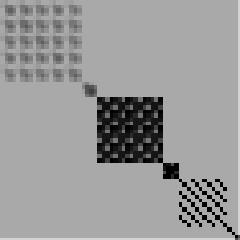
\includegraphics[scale=0.66]{figures/logo.pdf}};
\end{tikzpicture}
\end{center}

\vfill

\begin{abstract}
  Kronecker-factored approximate curvature \citep[KFAC,][]{martens2015optimizing} is arguably one of the most prominent curvature approximations in deep learning.
  Its applications range from optimization to Bayesian deep learning, training data attribution with influence functions, and model compression or merging.
  While the intuition behind KFAC is easy to understand, its implementation is tedious: It comes in many flavours, has common pitfalls when translating the math to code, and is challenging to test, which complicates ensuring a properly functioning implementation.
  Some of the authors themselves have dealt with these challenges and experienced the discomfort of not being able to fully test their code.
  Thanks to recent advances in understanding KFAC, we are now able to provide test cases and a recipe for a reliable KFAC implementation.
  \emph{This tutorial is meant as a ground-up introduction to KFAC.}
  In contrast to the existing work, our focus lies on providing both math and code side-by-side, and providing test cases based on latest insights into KFAC that are scattered throughout the literature.
  We hope this tutorial provides a contemporary view onto KFAC that
  allows beginners to gain a deeper understanding of this curvature approximation, while lowering the barrier to its implementation, extension, and usage in practise.
\end{abstract}

\vfill

\paragraph{Version:} \today\,(v1.0.0)

\paragraph{About the length of this document.}
Before you close this document because of its page number, take a moment to scroll through it.
You will realize that the effective length of this tutorial is much shorter than suggested by its page number.
This is because \emph{we use an experimental two-column layout which presents text and code in parallel} and leads to a good amount of white space.
We deliberately chose this format because it allows to explicitly spell out the math in code.

\paragraph{Follow along in code.} The \LaTeX\,\& Python source code is available at \href{\repourl}{\texttt{github.com/f-dangel/kfac-tutorial}}.
This allows you to run the code as you read:
Clone the repository and follow the installation instructions.
You can then run each snippet from the repository root, for instance by calling \texttt{python kfs/basics/forward\_pass.py}.
If you find typos or have suggestions for improving improving explanations, math, or code, please open issues and pull requests.
In doing so, you are contributing to making this tutorial a valuable reference for newcomers.

\vspace{\baselineskip}
%%% Local Variables:
%%% mode: latex
%%% TeX-master: "../main"
%%% End:

\clearpage

\tableofcontents
\clearpage

\section{Preface}
This is an attempt to bundle scattered knowledge about KFAC into a single document, explain all the technicalities and pitfalls, and present tests to ensure bug-free implementations.

Should answer the following questions:
\begin{itemize}
\item Why do we need this tutorial?
\item Why is this not a Jupyter notebook?
\item What do we gain by explaining KFAC bottom-up?
\item What ML framework do we use and why?
\item What are we \emph{not} doing (e.g.\,building an optimizer)?
\end{itemize}

We use PyTorch~\cite{paszke2019pytorch} and implement everything using \texttt{torch.nn} rather than a functional formulation as we feel that many deep learning practitioners are more familiar with this style.
There could be a JAX or functorch version, too.

\begin{itemize}
\item KFAC approximates the Fisher, which is an outer product of gradients. The gradients involve the output-parameter Jacobian of a weight, which has Kronecker structure,
  \begin{align}
    \jac_{\mW}(\mW \vx) = \vx^{\top} \otimes \mI\,.
  \end{align}
  This implies that the Fisher contains terms of the following form, where $\bullet$ is a placeholder for some matrix,
  \begin{align}
    \left(
    \vx^{\top}\otimes \mI
    \right)^{\top}
    \bullet
    \left(
    \vx^{\top}\otimes \mI
    \right)\,.
  \end{align}

\item The goal is to build up to an abstract general formulation of KFAC.
  Given a compute graph which uses the operations $\vx, \mW \mapsto \mW x$, potentially in multiple places, define a Kronecker approximation of the Fisher.
  Also to show the different degrees of freedom: treating weights \& biases jointly/separately, using reduce versus expand approximation, and treating weight tying, i.e.
  multi-usage of $\mW$.

\end{itemize}
TODO Should mention somewhere that many of the provided examples are already discussed in Felix's PhD thesis~\cite{dangel2023backpropagation}.
%%% Local Variables:
%%% mode: latex
%%% TeX-master: "../main"
%%% End:

\clearpage

\columnratio{0.42}
\begin{paracol}{2}
  \section{Basics}
  \subsection{Empirical risk minimization \& Maximum Likelihood Estimation}

\subsubsection{Deep neural networks}

\subsubsection{Probabilistic interpretation}


\begin{align}
  \gL(\vtheta) &= \sum_{n=1}^N \ell(\vtheta, \vx_n, \vy_n)
  \\
               &=
                 \sum_{n=1}^N c(f(\vtheta, \vx_n), \vy_n)
\end{align}

\switchcolumn[0]

\blindtext

\switchcolumn[1]

\switchcolumn[0]* % sync

\blindtext

\subsection{Derivatives \& Automatic Differentiation}

\begin{caveat}
  In deep learning, we often work with matrices, or higher-dimensional tensors.
  We want to use matrix linear algebra expressions to avoid using heavy index notation.
  This can be achieved by flattening all tensors back into vectors and re-using definitions derivatives from the vector case.
  However, we must be careful when translating the results back to the tensor format, as the translation process depends on the flattening convention.
  Classically, the mathematical derivations prefer a \emph{different} flattening scheme than the one used in deep learning libraries.
\end{caveat}

\switchcolumn[0]*
\subsubsection{Flattening}
There are many ways to flatten the entries of a tensor into a vector.
The two by far most common conventions are (i) last-varies-fastest ($\cvec$) and (ii) first-varies-fastest ($\rvec$).
Their names are easy to remember from their action on a matrix (see \Cref{ex:flattening}): $\cvec$-flattening concatenates columns into a vector (column flattening); $\rvec$-flattening concatenates rows into a vector (row flattening).
Column-flattening is popular in mathematical presentations, while row-flattening is popular in deep learning libraries which lay out tensors in row-major format in memory.
To see their differences, we will implement both.

For arbitrary tensors, we can generalize the matrix flattenings by ordering entries such that either their last index ($\cvec$, \Cref{def:cvec}) or first index ($\rvec$, \Cref{def:rvec}) varies fastest:

\switchcolumn[1]*
\codeblock{basics/flattening}
\switchcolumn[0]

\begin{setup}\label{setup:flattening}
  Let $\tA \in \sR^{N_1 \times \dots \times N_A}$ be a tensor of rank $A$ whose entries are indexed through a tuple $(n_1, \dots, n_A)$ where $n_a \in \{1, \dots, N_a\}$.
\end{setup}
\begin{definition}[$\cvec$, \Cref{flattening}]\label{def:cvec}
  The first-varies-fastest flattening of $\tA$ from \Cref{setup:flattening} is
  \begin{align*}
    \cvec(\tA) =
    \begin{pmatrix}
      \etA_{1,1,\dots,1} \\
      \etA_{2,1,\dots,1} \\
      \vdots \\
      \etA_{N_1,1,\dots,1} \\
      \etA_{1,2,\dots,1} \\
      \vdots \\
      \etA_{N_1,2,\dots,1} \\
      \vdots \\
      \etA_{N_1,N_2,\dots,N_A}
    \end{pmatrix}
    \in \sR ^{N_1 \cdots N_A}\,.
  \end{align*}
\end{definition}

\begin{definition}[$\rvec$, \Cref{flattening}]\label{def:rvec}
  The last-varies-fastest flattening of $\tA$ from \Cref{setup:flattening} is
  \begin{align*}
    \rvec(\tA) =
    \begin{pmatrix}
      \etA_{1,\dots,1,1} \\
      \etA_{1,\dots,1,2} \\
      \vdots \\
      \etA_{1,\dots,1,N_A} \\
      \etA_{1,\dots,2,1} \\
      \vdots \\
      \etA_{1,\dots,2,N_A} \\
      \vdots \\
      \etA_{N_1,\dots,N_{A-1},N_A}
    \end{pmatrix}
    \in \sR ^{N_A \cdots N_1}\,.
  \end{align*}
\end{definition}

In code, we will sometimes require partial flattening of a sub-set of contiguous indices, instead of all indices.
The definitions are analogous, but the flattened indices are surrounded by static ones.

\begin{example}[Matrix flattening, \Cref{flattening}]\label{ex:flattening}
  For a matrix
  \begin{equation*}
    \mA = \begin{pmatrix} 1 & 2 \\ 3 & 4 \end{pmatrix}
  \end{equation*}
  we have
  \begin{equation*}
    \rvec(\mA)
    =
    \begin{pmatrix}
      1 \\ 2 \\ 3 \\ 4
    \end{pmatrix}\,,
    \qquad
    \cvec(\mA)
    =
    \begin{pmatrix}
      1 \\ 3 \\ 2 \\ 4
    \end{pmatrix}\,.
  \end{equation*}
\end{example}
%%% Local Variables:
%%% mode: latex
%%% TeX-master: "../main"
%%% End:


\switchcolumn[0]*
\subsubsection{Jacobians, JVP, VJPs}
Building up to curvature approximations that tackle the approximation of second-order partial derivatives, we start with first-order derivatives.
These are collected into a matrix called the Jacobian, which depends on the flattening convention.
We can multiply with the Jacobian and its transpose via automatic differentiation, without building up the matrix in memory.
These operations are called vector-Jacobian products (VJPs) and Jacobian-vector products (JVPs), respectively.

Machine learning libraries like JAX and PyTorch offer routines for computing Jacobians, VJPs, and JVPs.
However, their interface is functional.
Here, we provide an alternative implementation that accepts nodes of a computation graph rather than functions as input and will be beneficial for modular implementations of neural networks, as we consider later.
We also provide examples for important Jacobians, namely the output-parameter Jacobian of an affine map, \ie a linear layer.
These Jacobians exhibit Kronecker structure, which is the foundation for the `K' in KFAC.
We verify this structure numerically and observe how the flattening convention affects it.

\begin{setup}[Vector-to-vector function]\label{setup:vector_to_vector_function}
  Let function $f: \sR^A \to \sR^B, \va \mapsto \vb = f(\va)$ denote a vector-to-vector function.
\end{setup}

\begin{definition}[Jacobian of a vector-to-vector function]\label{def:vector_jacobian}
  The Jacobian of a vector-to-vector function $f$ from \Cref{setup:vector_to_vector_function}, $\jac_{\va}\vb \in \sR^{B \times A}$, collects the first-order partial derivatives into a matrix such that
  \begin{align*}
    [\jac_{\va} \vb]_{i,j} = \frac{\partial [f(\va)]_i}{\partial [\va]_j}\,.
  \end{align*}
\end{definition}
\Cref{def:vector_jacobian} is limited to vector-to-vector functions.
The more general Jacobian of a tensor-to-tensor function can be indexed with combined indices from the input and output domains:

\begin{setup}[Tensor-to-tensor function]\label{setup:jacobians}
  Consider a tensor-to-tensor function $f: \sR^{A_1 \times \dots \times A_N} \to \sR^{B_1 \times \dots \times B_M}, \tA \mapsto \tB = f(\tA)$ from a rank-$N$ tensor $\tA$ into a rank-$M$ tensor $\tB$.
\end{setup}

\begin{definition}[General Jacobian, \Cref{basics/jacobians}]\label{def:general_jacobian}
  The general Jacobian of $f$ from \Cref{setup:jacobians}, $\tJ_{\tB}\tA$, is a rank-$(M+N)$ tensor that collects the first-order partial derivatives such that
  \begin{align*}
    [\tJ_{\tA}\tB]_{\colored{i_1, \dots, i_M}, \colored[VectorPink]{j_1, \dots, j_N}}
    =
    \frac{\partial [f(\tA)]_{\colored{i_1, \dots, i_M}}}{\partial [\tA]_{\colored[VectorPink]{j_1, \dots, j_N}}}\,.
  \end{align*}
\end{definition}
For $M=N=1$, the general Jacobian reduces to the Jacobian of a vector-to-vector function from \Cref{def:vector_jacobian}.

\switchcolumn[1]*
\codeblock{basics/jacobian_products}
\switchcolumn[0]

\paragraph{Jacobian multiplication.} In practice, this general Jacobian can be prohibitively large and therefore one must almost always work with it in a matrix-free fashion, \ie through VJPs and JVPs.

\begin{definition}[Vector-Jacobian products (VJPs), \Cref{basics/jacobian_products}]\label{def:vjp}
  Given a tensor-to-tensor function $f$ from \Cref{setup:jacobians} and a tensor $\tV \in \sR^{B_1 \times \dots \times B_M}$ in the output domain, the vector-Jacobian product (VJP) $\tU$ of $\tV$ and $\tJ_{\tA}\tB$ lives in $f$'s input domain and follows by contracting the \colored{output indices},
  \begin{align*}
    & [\tU]_{j_1, \dots, j_N}
    \\
    & =
      \colored{\sum_{i_1, \dots, i_M}}
      [\tV]_{\colored{i_1, \dots, i_M}}
      [\tJ_{\tA}\tB]_{\colored{i_1, \dots, i_M}, j_1, \dots, j_N}\,.
  \end{align*}
\end{definition}
For $M=N=1$, $\tV, \tU \to \vv, \vu$ are column vectors, $\tJ_{\tA}\tB \to \jac_{\va}\vb$ is a matrix, and the VJP is $\vu^{\top} = \vv^{\top} (\jac_{\va}\vb)$ or $\vu = (\jac_{\va}\vb)^{\top} \vv$, \ie multiplication with the transpose Jacobian.

VJPs are at the heart of reverse-mode automatic differentiation, aka backpropagation (this is why $\tU$ is often called the \emph{pull-back} or \emph{backpropagation} of $\tV$ through $f$).
Therefore, they are easy to implement with standard functionality (\eg \texttt{autograd.grad} in PyTorch).

The other relevant contraction is between the Jacobian and a vector from the input domain:

\begin{definition}[Jacobian-vector products (JVPs), \Cref{basics/jacobian_products}]\label{def:jvp}
  Given a tensor-to-tensor function $f$ from \Cref{setup:jacobians} and a tensor $\tV \in \sR^{A_1 \times \dots \times A_N}$ in the input domain, the Jacobian-vector product (JVP) $\tU$ between $\tV$ and $\tJ_{\tA}\tB$ lives in $f$'s output domain and follows by contracting the \colored[VectorPink]{input indices},
  \begin{align*}
    & [\tU]_{j_1, \dots, j_M}
    \\
    & =
      \colored[VectorPink]{\sum_{i_1, \dots, i_N}}
      [\tJ_{\tA}\tB]_{j_1, \dots, j_M, \colored[VectorPink]{i_1, \dots, i_N}}
      [\tV]_{\colored[VectorPink]{i_1, \dots, i_N}}\,.
  \end{align*}
\end{definition}
For the vector case, $\tU, \tV, \tJ_{\tA}\tB \to \vu, \vv, \jac_{\va}\vb$, the JVP is $\vu = (\jac_{\va}\vb) \vv$, as suggested by its name.
JVPs are common in forward-mode automatic differentiation ($\tU$ is often called the \emph{pushforward} of $\tV$ through $f$).
Only recently has this mode garnered attention.
The current JVP functionality in ML libraries usually follows a functional API.
To obtain an implementation that accepts variables from a computation graph and is more compatible with the modular approach we chose in this tutorial, we can use a trick that implements a JVP using two VJPs \cite{townsend2017new}.

\switchcolumn[1]*
\begin{figure}[!h]
  \centering
  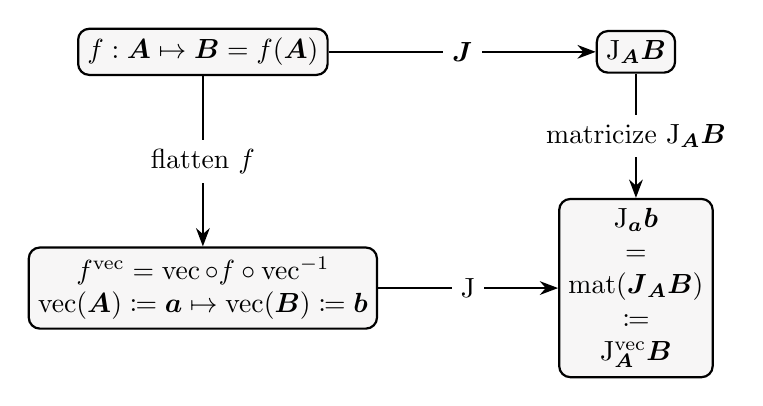
\begin{tikzpicture}[%
    % font=\scriptsize,%
    thick,
    box/.style = {rectangle, draw=black, rounded corners, fill=VectorGray!50},%%
    ]
    \node[box] (A) at (0,0) {$f: \tA \mapsto \tB = f(\tA)$};
    \node[box] (B) at (5.5,0) {$\jac_{\tA}\tB$};
    \node[box, align=center] (C) at (0,-3) {%
      $f^{\vec} = \vec \circ f \circ \vec^{-1}$\\%
      $\vec(\tA) \coloneq \va \mapsto \vec(\tB) \coloneq \vb$%
    };
    \node[box, align=center] (D) at (5.5,-3) {%
      $\jac_{\va} \vb$\\%
      $=$\\%
      $\mat(\tJ_{\tA}\tB)$\\%
      $\coloneq$\\%
      $\jac^{\vec}_{\tA}\tB$%
    };
    \draw[-Stealth] (A.east) -- node[fill=white] {$\tJ$} (B.west);
    \draw[-Stealth] (A.south) -- node[fill=white] {flatten $f$} (C.north);
    \draw[-Stealth] (C.east) -- node[fill=white] {$\jac$} (D.west);
    \draw[-Stealth] (B.south) -- node[fill=white] {matricize $\jac_{\tA}\tB$} (D.north);
  \end{tikzpicture}
  \caption{\textbf{Flattening and taking the Jacobian commute and lead to the same matricized Jacobian.}
    $\vec$ denotes one of the flattening conventions from \Cref{def:cvec,def:rvec}.
    $\mat$ denotes matricization (two partial flattenings for row and column dimensions, respectively).}\label{fig:commutative-diagram-jacobian}
\end{figure}
\switchcolumn[0]

\paragraph{Matricization.}
Jacobian products are efficient, but somewhat abstract to work with, as we cannot `touch' the full tensor.
Often, we would also like to think about this tensor as a matrix to be able to present derivations in linear algebra notation.

We can reduce the general Jacobian tensor back to the Jacobian matrix in two different ways: We can either (i) directly matricize the tensor, or (ii) `flatten' the function $f \to f^{\vec}$ such that it consumes and produces vectors, then compute its Jacobian.
Both ways and their resulting Jacobian matrices depend on the flattening convention we choose.
The following definitions are consistent in the sense that both of the aforementioned approaches yield the same result, illustrated by this commutative diagram in \cref{fig:commutative-diagram-jacobian}.


\switchcolumn[1]
\codeblock{basics/jacobians}
\switchcolumn[0]

For this tutorial, the two matrices of interest are the $\cvec$- and $\rvec$-Jacobians.
The $\cvec$-Jacobian is used in mathematical derivations in the literature.
The $\rvec$-Jacobian is common in code.

\begin{definition}[$\cvec$-Jacobian, \Cref{basics/jacobians}]\label{def:cvec_jacobian}
  For a tensor-to-tensor function $f$ from \Cref{setup:jacobians}, its $\cvec$-Jacobian $\jac^{\cvec}_{\tA}\tB \in \sR^{A_N \cdots A_1 \times B_M \cdots B_1}$ is attained by flattening the input and output tensors with $\cvec$ and applying the Jacobian definition for vectors,
  \begin{align*}
    [\jac^{\cvec}_{\tA}\tB]_{i,j}
    =
    \frac{\partial [\cvec(f(\tA))]_i}{\partial [\cvec(\tA)]_j}\,.
  \end{align*}
\end{definition}

\begin{definition}[$\rvec$-Jacobian, \Cref{basics/jacobians}]\label{def:rvec_jacobian}
  For a tensor-to-tensor function $f$ from \Cref{setup:jacobians}, its $\rvec$-Jacobian $\jac^{\rvec}_{\tA}\tB \in \sR^{A_1 \cdots A_N \times B_1 \cdots B_M}$ is attained by flattening the input and output tensors with $\rvec$ and applying the Jacobian definition for vectors,
  \begin{align*}
    [\jac^{\rvec}_{\tA}\tB]_{i,j}
    =
    \frac{\partial [\rvec(f(\tA))]_i}{\partial [\rvec(\tA)]_j}\,.
  \end{align*}
\end{definition}

\paragraph{Example.} The two Jacobians usually differ from each other, albeit in subtle ways.
We highlight their differences on a linear layer, which will be useful later on when we discuss KFAC (\Cref{ex:linear_layer_jacobians}, numerically verified in \cref{basics/jacobians_linear_layer}).
This example reveals two insights:
\begin{itemize}
\item There is a Kronecker structure in the linear layers' Jacobian \wrt its weight.
  This structure is the foundation for the `K' in KFAC.

\item The order of Kronecker factors is reversed depending on the flattening scheme.
  Therefore, we need to be careful when translating results from one convention to the other.
\end{itemize}

\switchcolumn[1]
\begin{example}[$\cvec$- and $\rvec$-Jacobians of a linear layer \wrt its weights, \Cref{basics/jacobians_linear_layer}]\label{ex:linear_layer_jacobians}
  Consider an affine map with weight matrix $\mW \in \sR^{D_{\text{out}} \times D_{\text{in}}}$, bias vector $\vb \in \sR^{D_{\text{out}}}$, input vector $\vx \in \sR^{D_{\text{in}}}$ and output vector $\vz \in \sR^{D_{\text{out}}}$,
  \begin{align*}
    \vz
    \coloneqq
    \mW \vx + \vb
    =
    \begin{pmatrix}
      \mW & \vb
    \end{pmatrix}
    \begin{pmatrix}
      \vx \\ 1
    \end{pmatrix}
    \coloneqq
    \tilde{\mW}
    \tilde{\vx}\,.
  \end{align*}
  To express this operation as matrix-vector multiplication, we combine weight and bias into a single matrix $\tilde{\mW}$ and augment the input with a one, yielding $\tilde{\vx}$, to account for the bias contribution.

  The linear layer's $\cvec$-Jacobian \wrt the combined weight is
  \begin{align*}
    \jac^{\cvec}_{\tilde{\mW}}\vz
    =
    \tilde{\vx}^{\top}
    \otimes
    \mI_{D_{\text{out}}}\,.
  \end{align*}
  In contrast, the $\rvec$-Jacobian is
  \begin{align*}
    \jac^{\rvec}_{\tilde{\mW}}\vz
    =
    \mI_{D_{\text{out}}}
    \otimes
    \tilde{\vx}^{\top}\,,
  \end{align*}
  see \Cref{basics/jacobians_linear_layer}.
  Note that the order of Kronecker factors is \emph{reversed}, depending on the flattening scheme.
\end{example}
\switchcolumn[0]

\switchcolumn[1]
\codeblock{basics/jacobians_linear_layer}
\switchcolumn[0]


% NOTE This example is about weight sharing, which will not be part of the tutorial's
% first version.
\begin{comment}
  \begin{example}[$\cvec$- and $\rvec$-weight Jacobians of a linear layer with weight sharing]
    Consider the same affine map from above, but now processing multiple input vectors $\mX = \begin{pmatrix}\vx_1 & \dots & \vx_S\end{pmatrix} \in \sR^{D_{\text{in}}\times S}$, yielding a sequence $\mZ = \begin{pmatrix} \vz_1 & \dots & \vz_S\end{pmatrix} \in \sR^{D_{\text{out}}\times S}$ where each $\vz_s$ is produced like above.
    The parameters are \emph{shared} over all vectors in the input sequence.
    In matrix notation,
    \begin{align*}
      \mZ
      & \coloneqq
        \mW \mX + \vb \vone^{\top}_S
      \\
      & =
        \begin{pmatrix}
          \mW & \vb
        \end{pmatrix}
        \begin{pmatrix}
          \mX \\ \vone^{\top}_S
        \end{pmatrix}
        \coloneqq
        \tilde{\mW}
        \tilde{\mX}\,.
    \end{align*}
    The $\cvec$-Jacobian \wrt the combined weight is
    \begin{align*}
      \jac^{\cvec}_{\tilde{\mW}}\mZ
      =
      \tilde{\mX}^{\top}
      \otimes
      \mI_{D_{\text{out}}}\,.
    \end{align*}
    In contrast, the $\rvec$-Jacobian is
    \begin{align*}
      \jac^{\rvec}_{\tilde{\mW}}\mZ
      =
      \mI_{D_{\text{out}}}
      \otimes
      \tilde{\mX}^{\top}\,.
    \end{align*}
  \end{example}

  \switchcolumn[1]
  \codeblock{basics/jacobians_shared_linear_layer}
\end{comment}

%%% Local Variables:
%%% mode: latex
%%% TeX-master: "../main"
%%% End:


\switchcolumn[0]*
\subsubsection{Hessians, HVPs}
Now that we have covered first-order derivatives, let's move on to second-order derivatives and develop the necessary concepts to understand KFAC, as well as their implementation.
Second-order derivatives are collected into an object called \emph{the Hessian}.
For our purposes, it will be sufficient to consider the Hessian of functions producing a scalar-valued output.
Let's start with the definition of the Hessian of a vector-to-scalar function.

\begin{setup}[Vector-to-scalar function]\label{setup:vector_to_scalar_function}
  Let $\vf: \sR^A \to \sR, \va \mapsto b = f(\va)$ be a vector-to-scalar function.
\end{setup}

\begin{definition}[Hessian of a vector-to-scalar function]\label{def:vector_hessian}
  The Hessian of a vector-to-scalar function $f$ from \Cref{setup:vector_to_scalar_function} is a matrix $\hess_{\va}b \in \sR^{A \times A}$ collecting the second-order partial derivatives of $f$ into a matrix with
  \begin{align*}
    [\hess_{\va}b]_{i,j}
     & =
    \frac{\partial^2 b}{\partial [\va]_i \partial [\va]_j}\,.
  \end{align*}
\end{definition}
This definition is limited to functions with vector-valued arguments. The extension to tensor-to-scalar functions is straightforward; however, it yields a tensor that is less convenient to work with in terms of notation:

\begin{setup}[Tensor-to-scalar function]\label{setup:hessians}
  Consider a tensor-to-scalar function $f: \sR^{A_1 \times \dots \times A_N} \to \sR, \tA \mapsto b = f(\tA)$ from a rank-$N$ tensor $\tA$ into a scalar $b$.
\end{setup}

\begin{definition}[General Hessian of a tensor-to-scalar function, \Cref{basics/hessians}]\label{def:general_hessian}
  The general Hessian of $f$ from \Cref{setup:hessians}, $\tH_{\tA}b \in \sR^{A_1 \times \dots \times A_N \times A_1 \times \dots \times A_N}$, collects the second-order partial derivatives of $f$ into a tensor with
  \begin{align*}
     & [\tH_{\tA}b]_{\colored{i_1, \dots, i_N}, \colored[VectorPink]{j_1, \dots, j_N}}
    \\
     & =
    \frac{\partial^2 b}{\partial [\tA]_{\colored{i_1, \dots, i_N}} \partial [\tA]_{\colored[VectorPink]{j_1, \dots, j_N}}}\,.
  \end{align*}
\end{definition}

\switchcolumn[1]*
\codeblock{basics/hessian_product}
\switchcolumn[0]

\paragraph{Hessian multiplication.}
Just like for Jacobians, the Hessian tensor is usually too large to be stored in memory.
Hence, one usually works with it implicitly through matrix-vector products, which can be done without computing the Hessian:

\begin{definition}[Hessian-vector products (HVPs), \Cref{basics/hessian_product}]\label{def:hvp}
  Given a tensor-to-scalar function $f$ from \Cref{setup:hessians} and a tensor $\tV \in \sR^{A_1 \times \dots \times A_N}$ in the input domain, the Hessian-vector product (HVP) $\tU$ of $\tV$ with $\tH_{\tA}b$ is the result of contraction with one of the Hessian's \colored{input indices},
  \begin{align*}
     & [\tU]_{i_1, \dots, i_N}
    \\
     & =
    \colored{\sum_{j_1, \dots, j_N}}
    [\tH_{\tA}b]_{i_1, \dots, i_N, \colored{j_1, \dots, j_N}} [\tV]_{\colored{j_1, \dots, j_N}}\,.
  \end{align*}
\end{definition}
For the vector case $N=1$, we have $\tV, \tA, \tH_{\tA}b \to \vv, \va, \hess_{\va}b$ and $\tU \to \vu = \hess_{\va} b$ as suggested by the name`Hessian-vector product'.

One way to multiply by the Hessian uses the so-called Pearlmutter trick~\cite{pearlmutter1994fast}.
It relies on the fact that multiplication with higher-order derivatives can be done by nested first-order differentiation.
Hence, multiplication with the Hessian can be done with two VJPs (\Cref{basics/hessian_product}).
In fact, this snippet implements a slightly more general Hessian that can handle differentiating twice \wrt \emph{different}, in contrast to the same, arguments.
It is not essential for understanding KFAC, and we will only use it to visualize curvature matrices in \Cref{subsec:curvature-matrices}.
In the context of KFAC, we do not care about these mixed second-order derivatives.

\switchcolumn[1]
\begin{figure}[!h]
  \centering
  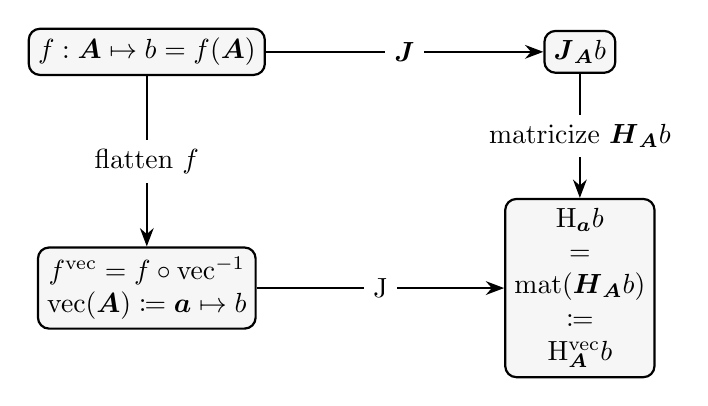
\begin{tikzpicture}[%
      % font=\scriptsize,%
      thick,
      box/.style = {rectangle, draw=black, rounded corners, fill=VectorGray!50},%%
    ]
    \node[box] (A) at (0,0) {$f: \tA \mapsto b = f(\tA)$};
    \node[box] (B) at (5.5,0) {$\tJ_{\tA}b$};
    \node[box, align=center] (C) at (0,-3) {%
      $f^{\vec} = f \circ \vec^{-1}$\\%
      $\vec(\tA) \coloneq \va \mapsto b$%
    };
    \node[box, align=center] (D) at (5.5,-3) {%
      $\hess_{\va} b$\\%
      $=$\\%
      $\mat(\tH_{\tA}b)$\\%
      $\coloneq$\\%
      $\hess^{\vec}_{\tA}b$%
    };
    \draw[-Stealth] (A.east) -- node[fill=white] {$\tJ$} (B.west);
    \draw[-Stealth] (A.south) -- node[fill=white] {flatten $f$} (C.north);
    \draw[-Stealth] (C.east) -- node[fill=white] {$\jac$} (D.west);
    \draw[-Stealth] (B.south) -- node[fill=white] {matricize $\tH_{\tA}b$} (D.north);
  \end{tikzpicture}
  \caption{\textbf{Flattening and taking the Hessian commute and lead to the same matricized Hessian.}
    $\vec$ denotes one of the flattening conventions from \Cref{def:cvec,def:rvec}.
    $\mat$ denotes matricization and involves two partial flattenings for row and column dimensions.}\label{fig:commutative-diagram-hessian}
\end{figure}
\switchcolumn[0]

\paragraph{Matricization:} For notational convenience, we will also define matricized versions of the general Hessian from \Cref{def:general_hessian}; the $\cvec$-, and $\rvec$-Hessian. Just like for the Jacobians, it does not matter whether we first flatten the function's input space then compute the Hessian, or compute the general Hessian then matricize it (\Cref{fig:commutative-diagram-hessian}).
The following definitions are consistent for both ways.

\switchcolumn[1]
\codeblock{basics/hessians}
\switchcolumn[0]

\begin{definition}[$\cvec$-Hessian, \Cref{basics/hessians}]\label{def:cvec_hessian}
  For a tensor-to-scalar function $f$ from \Cref{setup:hessians}, the $\cvec$-Hessian $\hess_{\tA}^{\cvec}b \in \sR^{A_N \cdots A_1 \times A_N \cdots A_1}$ results from flattening the input tensor with $\cvec$ and applying the Hessian from \Cref{def:vector_hessian},
  \begin{align*}
    [\hess^{\cvec}_{\tA}b]_{i, j}
     & =
    \frac{\partial^2 b}{\partial [\cvec(\tA)]_{i} \partial [\cvec(\tA)]_{j}}\,.
  \end{align*}
\end{definition}

\begin{definition}[$\rvec$-Hessian, \Cref{basics/hessians}]\label{def:rvec_hessian}
  For a tensor-to-scalar function $f$ from \Cref{setup:hessians}, the $\rvec$-Hessian $\hess_{\tA}^{\rvec}b \in \sR^{A_1 \cdots A_N \times A_1 \cdots A_N}$ results from flattening the input tensor with $\rvec$ and applying the Hessian from \Cref{def:vector_hessian},
  \begin{align*}
    [\hess^{\rvec}_{\tA}b]_{i, j}
     & =
    \frac{\partial^2 b}{\partial [\rvec(\tA)]_{i} \partial [\rvec(\tA)]_{j}}\,.
  \end{align*}
\end{definition}

Whenever we consider vector-to-scalar functions, both Hessians are identical, and we thus suppress the flattening scheme and write $\hess_{\va}b$.

\paragraph{Examples.}
Let's look at important Hessian examples we will return to later in the text.
We can use them to verify our Hessian implementation.

\switchcolumn[1]
\codeblock{basics/hessian_ce_loss}
\switchcolumn[0]

\begin{example}[Softmax cross-entropy loss Hessian, \Cref{basics/hessian_ce_loss}]\label{ex:hessian-crossentropyloss}
  Consider the softmax cross-entropy loss function between the vector-valued logits $\vf \in \sR^C$ and a class label $y \in \{1, \dots, C\}$ from \Cref{ex:cross_entropy_loss}:
  \begin{align*}
    c(\vf, y)
     & =
    -\log([\vsigma(\vf)]_y)\,.
  \end{align*}
  with $\vsigma(\vf) = \softmax(\vf) \in \sR^C$.
  Its Hessian \wrt $\vf$ is diagonal-minus-rank-one,
  \begin{align*}
    \hess_{\vf} c(\vf, y)
    =
    \diag(\vsigma) - \vsigma \vsigma^\top\,.
  \end{align*}
  See \eg~\citet{dangel2020modular} for a derivation.
\end{example}

\switchcolumn[1]
\codeblock{basics/hessian_mse_loss}

\switchcolumn[0]
\begin{example}[Square loss Hessian, \Cref{basics/hessian_mse_loss}]\label{ex:square_loss_hessian}
  Consider the square loss function between a vector-valued input $\vf \in \sR^C$ and its associated target $\vy \in \sR^C$ from \Cref{ex:square_loss}:
  \begin{align*}
    c(\vf, \vy)
     & =
    \frac{1}{2}\left\lVert
    \vf - \vy
    \right\rVert^2
    \\
     & =
    \frac{1}{2}(\vf - \vy)^{\top} \mI (\vf - \vy)\,.
  \end{align*}
  Its Hessian \wrt $\vf$ is the identity,
  \begin{align*}
    \hess_{\vf} \ell(\vf, \vy)
    =
    \mI_C\,.
  \end{align*}
\end{example}

%%% Local Variables:
%%% mode: latex
%%% TeX-master: "../main"
%%% End:


\switchcolumn[0]*
\subsection{Curvature Matrices in Deep Learning}
\subsubsection{The Hessian}

\subsubsection{The Generalized Gauss-Newton (GGN)}
Linearization
\subsubsection{The Fisher}
Probabilistic perspective

Explain type-1 versus type-2
\subsubsection{The Connection between GGN \& Fisher}
\subsubsection{The Empirical Fisher (EF)}

%%% Local Variables:
%%% mode: latex
%%% TeX-master: "../main"
%%% End:


  \switchcolumn[0]*
\end{paracol}

\clearpage
\begin{paracol}{1}
  \section{Cheatsheet: Basics}
  \begin{itemize}
\item Risk minimization and tractable empirical risk minimization (\Cref{subsec:empirical-risk-minimization})
  \begin{align*}
    \argmin_{\vtheta} \gL_{p_{\text{data}}(\rvx, \rvy)}(\vtheta)
    \qquad
    &\text{where}\qquad
      \gL_{p_{\text{data}}(\rvx, \rvy)}(\vtheta) \coloneq \E_{(\vx, \vy) \sim p_{\text{data}}(\rvx, \rvy)}
      \left[
      c(f(\vx, \vtheta), \vy)
      \right]
    &\text{(intractable)}
      \shortintertext{(use empirical density $p_{\sD}(\rvx, \rvy) = \frac{1}{N} \sum_n \delta(\rvx - \vx_n) \delta(\rvy - \vy_n)$ from data $\sD = \{ (\vx_n, \vy_n) \sim p_{\text{data}} \mid n=1, \dots, N \}$)}
      \argmin_{\vtheta} \gL_{\sD}(\vtheta)
      \qquad
    &\text{where}\qquad
      \gL_{\sD}(\vtheta) \coloneq R \sum_{n=1}^N c(f(\vx_n; \vtheta), \vy_n)\,.
    &\text{(tractable)}
  \end{align*}
  (changing the reduction factor $R$ does not change the optimization problem's solution)

\item Common criterion functions and their reduction constants (\Cref{ex:square_loss,ex:cross_entropy_loss})
  \begin{align*}
    &\begin{matrix}
      \text{Square loss}
      \\
      \text{(\texttt{MSELoss})}
    \end{matrix}
      \qquad
    &c(\vf, \vy) = \frac{1}{2} \left\lVert \vf - \vy \right\rVert_2^2\,,
      \qquad
    &R =
      \begin{cases}
        2 & \text{\texttt{reduction="sum"}} \\
        \frac{2}{N \dim(\vy)} & \text{\texttt{reduction="mean"}}
      \end{cases}
    \\
    &\begin{matrix}
      \text{Softmax cross-entropy loss}\\
      \text{(\texttt{CrossEntropyLoss})}
    \end{matrix}
      \qquad
    &c(\vf, y) = - \log( [\softmax(\vf)]_y)\,,
      \qquad
    &R =
      \begin{cases}
        1 & \text{\texttt{reduction="sum"}} \\
        \frac{1}{N \dim(\vf)} & \text{\texttt{reduction="mean"}}
      \end{cases}
  \end{align*}

\item Probabilistic interpretation of a neural net: Parameterize $p(\rvx, \rvy \mid \vtheta) = p_{\text{data}}(\rvx) p(\rvy \mid \rvx, \vtheta) = p_{\text{data}}(\rvx) r(\rvy \mid f(\rvx, \vtheta))$
  \begin{align*}
    \argmin_{\vtheta} \mathrm{KL}( p_{\text{data}}(\rvx, \rvy) \mid\mid p(\rvx, \rvy \mid \vtheta) )
    \quad\Leftrightarrow\quad
    &\argmin_{\vtheta} \E_{p_{\text{data}}(\rvx)} \E_{r(\rvy \mid \rvx, \vtheta)} \left[
      - \log r(\rvy \mid f(\rvx, \vtheta))
      \right]
    &\text{(intractable)}
      \shortintertext{(use empirical density to make tractable)}
      \qquad
    &\argmin_{\vtheta} - R \sum_{n=1}^N \log r(\rvy=\vy_n \mid f(\rvx=\vx_n, \vtheta))
    &\text{(tractable)}
  \end{align*}

\item Common criteria are negative log-likelihoods: $c(\vf, \vy) = - \log r(\rvy=\vy \mid f(\rvx, \vtheta) = \vf)$ (\Cref{ex:square_loss_probabilistic,ex:cross_entropy_loss_probabilistic})
  \begin{align*}
    &\text{Square loss (\texttt{MSELoss})}
      \qquad
    &r(\rvy \mid \vf) = \gN( \rvy \mid \vmu = \vf, \mSigma = \mI)
    \\
    &\text{Softmax cross-entropy loss (\texttt{CrossEntropyLoss})}
      \qquad
    &r(\ry \mid \vf) = \gC( \ry \mid \vsigma = \softmax(\vf))
  \end{align*}

\item Shorthands: Per-datum prediction $\vf_n(\vtheta) = f(\vx_n, \vtheta)$, criterion $c_n(\vf_n) = c(\vf_n, \vy_n)$, and loss $\ell_n(\vtheta) = c_n(\vf_n(\vtheta))  $

\item Net Jacobian $\jac_{\vtheta}\vf \in \sR^{\dim(\gF) \times D}$, $[\jac_{\vtheta} \vf]_{i,j} = \frac{\partial [\vf]_i}{\partial [\vtheta]_j}$, criterion Hessian $\hess_{\vf} c \in \sR^{\dim(\gF) \times \dim(\gF)}$, $[\hess_{\vf}c]_{i,j} = \frac{\partial^2 c}{\partial [\vf]_i \partial [\vf]_j}$

\item Hessian, generalized Gauss-Newton, type-II/I/empirical Fishers ($\vf_n \coloneq f(\vx_n, \vtheta)$, $\rvf = f(\rvx, \vtheta)$, $\tilde{\vy}_{n,m} \sim r(\rvy \mid \rvf = \vf_n)$)
  \begin{align*}
    \hess_{\vtheta} \gL(\vtheta)
    &= R \sum_{n=1}^N \hess_{\vtheta} c(\vf_n, \vy_n)
      = -R \sum_{n=1}^N \hess_{\vtheta} \log r(\rvy = \vy_n \mid \rvf = \vf_n)
    \\
    \mG(\vtheta)
    &= R \sum_{n=1}^N
      \jac_{\vtheta} \vf_n^{\top}
      \left(
      \hess_{\vf_n} c(\vf_n, \vy_n)
      \right)
      \jac_{\vtheta} \vf_n
      =
      R \sum_{n=1}^N
      \jac_{\vtheta} \vf_n^{\top}
      \left(
      -\hess_{\vf_n} \log r(\rvy = \vy_n \mid \rvf = \vf_n)
      \right)
      \jac_{\vtheta} \vf_n
    \\
    \mF^{\text{II}}(\vtheta)
    &=
      \lim_{M \to \infty}
      \frac{R}{M}
      \sum_{n=1}^N
      \jac_{\vtheta} \vf_n^{\top}
      \left[
      \hess_{\vf_n}(\underbrace{- \log r(\rvy = \tilde{\vy}_{n,m} \mid \rvf = \vf_n)}_{= c(\vf_n, \tilde{\vy}_{n,m})} )
      \right]
      \jac_{\vtheta} \vf_n
    \\
    \mF^{\text{I}}(\vtheta)
    &=
      \lim_{M \to \infty}
      \frac{R}{M}
      \sum_{n=1}^N
      \jac_{\vtheta} \vf_n^{\top}
      \left[
      -\nabla_{\vf_n} \log r(\rvy = \tilde{\vy}_{n,m} \mid \rvf = \vf_n)
      (-\nabla_{\vf_n} \log r(\rvy = \tilde{\vy}_{n,m} \mid \rvf = \vf_n))^{\top}
      \right]
      \jac_{\vtheta} \vf_n
    \\
    \mE(\vtheta)
    &=
      R
      \sum_{n=1}^N
      (\nabla_{\vtheta} c(\vf_n, \vy_n))
      (\nabla_{\vtheta} c(\vf_n, \vy_n))^{\top}
  \end{align*}
  \begin{itemize}
  \item In expectation notation (coloured parts coincide for the above criterion functions, hence GGN = Fisher)
    \begin{align*}
      \hess_{\vtheta} \gL_{\sD}(\vtheta)
      &\propto
        \E_{p_{\sD}(\rvx)}
        \E_{p_{\sD}(\rvy \mid \rvx)}
        \left[
        -\hess_{\vtheta} \log r(\rvy \mid \rvf)
        \right]
      \\
      \mF(\vtheta)
      &\propto
        \E_{p_{\sD}(\rvx)}
        \E_{r(\rvy \mid \rvf)}
        \left[
        -\hess_{\vtheta} \log r(\rvy \mid \rvf)
        \right]
      \\
      \mG(\vtheta)
      &\propto
        \E_{p_{\sD}(\rvx)}
        \left[
        \jac_{\vtheta} \rvf^{\top}
        \textcolor{VectorBlue}{
        \E_{p_{\sD}(\rvy \mid \rvx)}
        \left[
        -\hess_{\rvf} \log r(\rvy \mid \rvf)
        \right]
        }
        \jac_{\vtheta} \rvf
        \right]
      \\
      \mF^{\text{II}}(\vtheta)
      &\propto
        \E_{p_{\sD}(\rvx)}
        \left[
        \jac_{\vtheta} \rvf^{\top}
        \textcolor{VectorBlue}{
        \E_{r(\rvy \mid \rvf)}
        \left[
        -\hess_{\rvf} \log r(\rvy \mid \rvf)
        \right]
        }
        \jac_{\vtheta} \rvf
        \right]
      \\
      \mF^{\text{I}}(\vtheta)
      &\propto
        \E_{p_{\sD}(\rvx)}
        \left[
        \jac_{\vtheta} \rvf^{\top}
        \textcolor{VectorBlue}{
        \E_{r(\rvy \mid \rvf)}
        \left[
        -\nabla_{\rvf} \log r(\rvy \mid \rvf)
        (
        -\nabla_{\rvf} \log r(\rvy \mid \rvf)
        )^{\top}
        \right]
        }
        \jac_{\vtheta} \rvf
        \right]
      \\
      \mE(\vtheta)
      &\propto
        \E_{p_{\sD}(\rvx)}
        \left[
        \jac_{\vtheta} \rvf^{\top}
        \E_{p_{\sD}(\rvy \mid \rvx)}
        \left[
        -\nabla_{\rvf} \log r(\rvy \mid \rvf)
        (
        -\nabla_{\rvf} \log r(\rvy \mid \rvf)
        )^{\top}
        \right]
        \jac_{\vtheta} \rvf
        \right]
    \end{align*}
  \end{itemize}
\item Gradients (\Cref{ex:square-loss-gradient,ex:cross-entropy-loss-gradient}), Hessians (\Cref{ex:hessian-crossentropyloss,ex:square_loss_hessian}), and symmetric Hessian decompositions (\Cref{ex:mseloss_hessian_factorization,ex:crossentropyloss_hessian_factorization}) of criterion functions
  \begin{align*}
    &
      \qquad&\nabla_{\vf} c(\vf, \vy)
              \qquad&\hess_{\vf} c(\vf, \vy)
                      \qquad&\mS,\, \mS \mS^{\top} = \hess_{\vf} c(\vf, \vy)
    \\
    &
      \begin{matrix}
        \text{Square loss}\\
        \text{(\texttt{MSELoss})}
      \end{matrix}
    & \vf - \vy
      \qquad& \mI
              \qquad& \mI
    \\
    &
      \begin{matrix}
        \text{Softmax cross-entropy loss}\\
        (\text{\texttt{CrossEntropyLoss}})\\
        (\vsigma = \softmax(\vf))
      \end{matrix}
      \qquad& \vsigma - \onehot(y)
              \qquad& \diag(\vsigma) - \vsigma \vsigma^{\top}
                      \qquad& \diag(\sqrt{\vsigma}) - \vsigma \sqrt{\vsigma}^{\top}
  \end{align*}
\end{itemize}
%%% Local Variables:
%%% mode: latex
%%% TeX-master: "../main"
%%% End:

\end{paracol}
\clearpage

\begin{paracol}{2}
  \section{KFAC for Linear Layers}
  The goal of this section should be to describe the KFAC approximation from~\cite{martens2015optimizing}

Let's consider the GGN for a linear layer with weights $\mW$, input vector $\vx$, and output vector $\vz = \mW \vx$ (suppressing layer indices for simplicity). Let's also assume $\cvec$-flattening, as usually done by the literature and make use of the output-parameter Jacobian of a linear layer (remember Example ??)
\begin{align*}
  \ggn_{\mW} \gL_{\sD}
  &=
    R
    \sum_n \sum_c
    (\jac^{\rvec}_{\mW}\vz_n)^{\top}
    (\jac^{\rvec}_{\vz_n}\vf_n)^{\top}
    \blacktriangle_{n,c}
    \blacktriangle_{n,c}^{\top}
    (\jac^{\rvec}_{\vz_n}\vf_n)
    (\jac^{\rvec}_{\mW}\vz_n)
  \\
  \shortintertext{
  (introduce $\vb_{n,c} \coloneq (\jac^{\rvec}_{\vz_n}\vf_n)^{\top} \blacktriangle_{n,c}$ for the layer output gradient)
  }
  &=
    R
    \sum_n \sum_c
    (\jac^{\rvec}_{\mW}\vz_n)^{\top}
    \vb_{n,c} \vb_{n,c}^{\top}
    (\jac^{\rvec}_{\mW}\vz_n)
    \shortintertext{Insert the linear layer's Jacobian}
  &=
    R
    \sum_n \sum_c
    (\vx_n \otimes \mI_{D_{\text{out}}})
    \vb_{n,c} \vb_{n,c}^{\top}
    (\vx_n^{\top} \otimes \mI_{D_{\text{out}}})
  \\
  &=
    R
    \sum_c
    \sum_n
    \vx_n \vx_n^{\top}
    \otimes
    \vb_{n,c} \vb_{n,c}^{\top}
\end{align*}

The expectation approximation in KFAC is the following:
\begin{align}
  \sum_n \va_n\va_n^{\top} \otimes \vb_n \vb_n^{\top}
  \approx
  \left( \sum_n \va_n \va_n^{\top} \right)
  \otimes
  \frac{
  \left( \sum_n \vb_n \vb_n^{\top} \right)
  }{N}
\end{align}
Instead of summing Kronecker products, we first sum the individual factors, then take their Kronecker product and divide by the number of summands. The scaling is by convention absorbed into the gradient-based Kronecker factor.

Our discussion will heavily rely on regression settings with deep linear networks, i.e.\,MLPs that consist of dense layers without any non-linearities.
We think they are a great setup to understand the core approximations of KFAC, and verify them numerically through rigorous tests.

We will start with the KFAC-expand approximation, which corresponds to the seminal KFAC approximation proposed by~\citet{martens2015optimizing}. It was introduced for standard MLP settings where the linear layers do not exhibit weight sharing (and therefore no reductions over weight-shared axes).
We will then show how to extend KFAC-expand to the presence of weight sharing.

The discussion of KFAC-expand naturally leads to an alternative setting where weight sharing dimensions are reduced during a forward pass; the so-called reduce setting.
For this setting, KFAC is not well motivated as it has no limit in which it becomes exact.
As a solution, we will explain the alternative KFAC-reduce approximation, recently introduced by~\citet{eschenhagen2023kroneckerfactored}.

\subsection{KFAC-expand \& KFAC-reduce}

\begin{setup}[Linear layer inside a neural network]\label{setup:linear_layer}
  Consider a linear layer with weight $\mW \in \sR^{D_{\text{out}}\times D_{\text{in}}}$ and bias $\vb \in \sR^{D_{\text{out}}}$ inside a neural network.
  Further, assume the network's prediction feeds into a criterion function and we use a data set of $N$ points to compute an empirical risk (with a reduction factor $R$) whose curvature matrix $\mC(\vec \mW)$ we are interested in computing.

  For each datum $n$, the layer processes a sequence of $S$ vector inputs $\vx_{n,1}, \dots, \vx_{n,S} \in \sR^{D_{\text{in}}}$ into a sequence of $S$ vector outputs $\vz_{n,1}, \dots, \vz_{n,S} \in sR^{D_{\text{out}}}$ where $\vz_{n,s} = \mW \vx_{n,s} + \vb$.
  Equivalently, we can express the forward pass by
  \begin{align*}
    \mZ_n
    &=
      \mW \mX_n + \vb \vone_S^{\top}
      \shortintertext{where}
      \mX_n
    &=
      \begin{pmatrix} \vx_{n,1} & \ldots & \vx_{n,S} \end{pmatrix}
      \in \sR^{D_{\text{in}} \times S}\,,
    \\
    \mZ_n
    &=
      \begin{pmatrix} \vz_{n,1} & \ldots & \vz_{n,S} \end{pmatrix}
      \in \sR^{D_{\text{out}} \times S}\,.
  \end{align*}
  Denote $\mF_n \in \sR^{C \times S'}$ the network's prediction on datum $n$ where $S' \neq S$ in general, but usually $S' \in \{1, S\}$.
  For each vector $\blacktriangle_{n,c} \in \sR^{C \times S'}$ backpropagated by KFAC,
  define the errors arriving at the layer's output as $\vg_{n,s,c} = (\jac^{\vec}_{\vz_{n,s}} \mF_n)^{\top} \blacktriangle_{n,c} \in \sR^{D_{\text{out}}\times S}$. These vectors do not depend on the flattening scheme because the contracted dimensions are summed out. We can group them into a matrix-values layer output gradient
  \begin{align*}
    \mG_{n,c}
    =
    \begin{pmatrix}
      \vg_{n,1,c} & \ldots & \vg_{n,S,c}
    \end{pmatrix}
    \in \sR^{D_{\text{out}} \times S}\,.
  \end{align*}
\end{setup}

If we apply this approximation to the above, we obtain
\begin{align*}
  \kfac(\cvec \mW)
  &=
    \mA \otimes \mB
  \\
  \kfac(\rvec \mW)
  &=
    \mB \otimes \mA
    \shortintertext{where}
    \mA
  &=
    R
    \sum_n
    \vx_n \vx_n^{\top}
  \\
  \mB
  &=
    \frac{
    \left(
    \sum_n
    \sum_c
    \vb_{n,c} \vb_{n,c}^{\top}
    \right)
    }{N}
\end{align*}
Note that we absorbed the reduction factor of the loss into input-based factor.
Also note that the order of Kronecker factors changes depending on the flattening scheme.
The same equation holds if we treat weight and bias jointly, but we need to make the substitutions
\begin{align*}
  \mW \leftrightarrow \tilde{\mW}
  \quad
  \text{and}
  \quad
  \vx_n \leftrightarrow \begin{pmatrix} \vx_n \\ 1 \end{pmatrix}.
\end{align*}

\switchcolumn[1]
\codeblock{kfac/expand_Linear}
\switchcolumn[0]

\subsection{Tests}
When does this approximation become exact?
Generally speaking, it becomes exact whenever one or both of the Kronecker factors in ??
does not depend on $n$.

\begin{definition}[KFAC-expand for a linear layer, \Cref{kfac/expand_Linear}]\label{def:kfac_expand_linear}
  Consider a linear layer inside a neural network from \Cref{setup:linear_layer}.
  The KFAC-expand approximation of a curvature matrix w.r.t.\,the layer's weights is given by
  \begin{subequations}\label{eq:kfac_expand_linear}
    \begin{align}
      \begin{split}
        &\kfac_{\text{exp}}(\vec \mW) \approx \mC(\vec \mW)
        \\
        &\quad=
          \begin{cases}
            \mA_{\text{exp}} \otimes \mB_{\text{exp}} & \vec = \cvec
            \\
            \mB_{\text{exp}} \otimes \mA_{\text{exp}} & \vec = \rvec
          \end{cases}\,,
      \end{split}
    \end{align}
    with the input-based factor $\mA_{\text{exp}} \in \sR^{D_{\text{in}} \times D_{\text{in}}}$
    \begin{align}
      \mA_{\text{exp}} &= R \sum_{n=1}^N\sum_{s=1}^S \vx_{n,s} \vx_{n,s}^{\top}
                         \intertext{and the output-gradient-based factor $\mB_{\text{exp}} \in \sR^{D_{\text{out}} \times D_{\text{out}}}$}
                         \mB_{\text{exp}} &= \frac{1}{NS}\sum_{n=1}^N \sum_{s=1}^S \sum_c \vg_{n,s,c} \vg_{n,s,c}^{\top}\,.
    \end{align}
  \end{subequations}
\end{definition}

\switchcolumn[1]
\codeblock{kfac/reduce_Linear}
\switchcolumn[0]

\begin{definition}[KFAC-reduce approximation for a linear layer with weight sharing, \Cref{kfac/reduce_Linear}]\label{def:kfac_reduce_linear}
  Consider a linear layer inside a neural network from \Cref{setup:linear_layer}.
  The KFAC-reduce approximation for a curvature matrix w.r.t.\,the layer's weights is given by
  \begin{subequations}\label{eq:kfac_reduce_linear}
    \begin{align}
      \begin{split}
        &\kfac_{\text{red}}(\vec \mW) \approx \mC(\vec \mW)
        \\
        &\quad=
          \begin{cases}
            \mA_{\text{red}} \otimes \mB_{\text{red}} & \vec = \cvec
            \\
            \mB_{\text{red}} \otimes \mA_{\text{red}} & \vec = \rvec
          \end{cases}\,,
      \end{split}
    \end{align}
    with the input-based factor $\mA_{\text{red}} \in sR^{D_{\text{in}}\times D_{\text{in}}}$
    \begin{align}
      \begin{split}
        \mA_{\text{red}}
        &=
          R \sum_{n=1}^N
          \left( \sum_{s=1}^S \vx_{n,s} \right)
          \left( \sum_{s'=1}^S \vx_{n,s'} \right)^{\top}
        \\
        &=
          R \sum_{n=1}^N
          \left( \mX_n \vone_S \right)
          \left( \mX_n \vone_S \right)^{\top}
      \end{split}
      \intertext{and the output-gradient-based factor $\mB_{\text{red}} \in \sR^{D_{\text{out}}\times D_{\text{out}}}$}
      \begin{split}
        \mB_{\text{red}}
        &=
          \frac{1}{N S^2} \sum_{n=1}^N \sum_c
        \\
        &\qquad
          \left( \sum_{s=1}^S \vg_{n,s,c} \right)
          \left( \sum_{s'=1}^S \vg_{n,s',c} \right)^{\top}
        \\
        &= \frac{1}{N S^2} \sum_{n=1}^N \sum_c
          \left(\mG_{n,c} \vone_S \right)
          \left(\mG_{n,c} \vone_S \right)^{\top}
      \end{split}
    \end{align}
  \end{subequations}
\end{definition}

Comments on \Cref{def:kfac_reduce_linear,def:kfac_expand_linear}:
\begin{itemize}

\item The main difference between KFAC-expand and KFAC-reduce is how they treat the shared dimension.
  KFAC-expands treats the shared dimension independently and like a batch dimension.
  KFAC-reduce first accumulates the layer inputs and output-gradients over their shared dimension.
  In the absence of weight sharing, $S=1$, both approximations are equivalent.

\item Depending on which vectors we choose for backpropagation, we obtain the type-II, MC, empirical, and input-only KFAC-expand/reduce flavours $\kfac_{\text{red, exp}}^{\text{II}}$, $\kfac_{\text{red, exp}}^{\text{MC}}$, $\kfac_{\text{red, exp}}^{\text{E}}$ and $\kfac_{\text{red,exp}}^{\text{IO}}$.

\item If we treat weight and bias jointly via $\tilde{\mW} = \begin{pmatrix} \mW & \vb \end{pmatrix} \in \sR^{D_{\text{out}}\times (D_{\text{in}}+1)} $, we need to make the following substitutions in \Cref{eq:kfac_expand_linear} and $\mA_{\text{exp, red}} \in \sR^{(D_{\text{in}}+1) \times (D_{\text{in}}+1)}$:
  \begin{align*}
    \mW \leftrightarrow \tilde{\mW}
    \quad
    \text{and}
    \quad
    \vx_{n,s} \leftrightarrow \begin{pmatrix} \vx_{n,s} \\ 1 \end{pmatrix}\,.
  \end{align*}

\item By convention, the reduction factor $R$ is absorbed into the input-based Kronecker factor.
  This, as well as the summation over $c$, is done by the scaffold in \Cref{kfac/scaffold} and not by the layer-specific implementations in \Cref{kfac/expand_Linear,kfac/reduce_Linear} because the layer has no knowledge of $R$.
  This guarantees that we can safely set the output-gradient-based factor to the identity matrix for the input-only variation and still be able to recover the correct curvature matrix in special cases, even when changing the loss function's reduction.
\end{itemize}

\subsection{Algebraic Structure of a Curvature Matrix}
To try to get an intuition for the approximations introduced in the previous sections, let's take a closer look at the equation for a curvature matrix w.r.t.\,a linear layer inside a neural network from \Cref{setup:linear_layer},
\begin{align*}
  &\mC( \vec \mW)
  \\
  &=
    R\sum_{n=1}^N \sum_c
    (\jac_{\mW}^{\vec}\mZ_n)^{\top}
    (\jac_{\mZ_n}^{\vec}\mF_n)^{\top}
    (\vec \blacktriangle_{n,c})
  \\
  &\qquad\quad
    (\vec \blacktriangle_{n,c})^{\top}
    (\jac_{\mZ_n}^{\vec}\mF_n)
    (\jac_{\mW}^{\vec}\mZ_n)
  \\
  &=
    R\sum_{n=1}^N \sum_c \sum_{s=1}^S
    (\jac_{\mW}^{\vec}\vz_{n,s})^{\top}
    (\jac_{\vz_{n,s}}^{\vec}\mF_n)^{\top}
    (\vec \blacktriangle_{n,c})
  \\
  &\qquad\quad
    (\vec \blacktriangle_{n,c})^{\top}
    (\jac_{\vz_{n,s}}^{\vec}\mF_n)
    (\jac_{\mW}^{\vec}\vz_{n,s})
    \intertext{where we simply extracted the summation over the shared dimension by taking Jacobians w.r.t.\,the vectors in a sequence.
    Let's introduce the shortcut $\vg_{n,s,c} = (\jac_{\vz_{n,s}}^{\vec}\mF_n)^{\top} (\vec \blacktriangle_{n,c})$ for the gradient arriving at the layer's output for each vector of the sequence.
    It does not depend on $\vec$.}
  &=
    \sum_{n=1}^N \sum_c \sum_{s=1}^S
    (\jac_{\mW}^{\vec}\vz_{n,s})^{\top}
    \vg_{n,s,c}
    \vg_{n,s,c}^{\top}
    (\jac_{\mW}^{\vec}\vz_{n,s})
\end{align*}
Next, let's set $\vec = \cvec$ and insert the linear layer's output-weight Jacobian to get
\begin{align*}
  &\mC(\cvec \mW)
  \\
  &=
    R\sum_{n=1}^N \sum_c \sum_{s=1}^S
    \left( \vx_{n,s} \otimes \mI \right)
    \vg_{n,s,c}
    \vg_{n,s,c}^{\top}
    \left( \vx_{n,s}^{\top} \otimes \mI \right)
  \\
  &=
    R\sum_{n=1}^N \sum_c \sum_{s=1}^S
    \vx_{n,s} \vx_{n,s}^{\top} \otimes
    \vg_{n,s,c} \vg_{n,s,c}^{\top}
  \\
  &=
    R\sum_{n=1}^N \sum_c
    \left( \mX_{n} \otimes \mI \right)
    \cvec\mG_{n,c}
    (\cvec \mG_{n,c})^{\top}
    \left( \mX_{n}^{\top} \otimes \mI \right)
\end{align*}

The curvature matrix is a sum of Kronecker products.
We want to approximate this with a single Kronecker product.
To do that, we need to agree on a convention to carry out the sum over $n$ before taking the Kronecker product. We will use:
\begin{definition}[KFAC's expectation approximation]
  Consider two sets of $N$ vectors $\{\vx_{n}\}_{n=1}^N$ and $\{\vg_{n}\}_{n=1}^N$ where each $\vx_n$ is input-based and each $\vg_n$ is output-gradient-based.
  KFAC approximates the summed Kronecker products of the self-outer products $\vx_n \vx_n^{\top} \otimes \vg_n \vg_n^{\top}$ as a single Kronecker products using the following expectation approximation:
  \begin{subequations}\label{eq:expectation_approximation}
    \begin{align}
      \begin{split}
        &\sum_{n=1}^{\textcolor{VectorOrange}{N}} \vx_n\vx_n^{\top} \otimes \vg_n \vg_n^{\top}
        \\
        &\qquad\approx
          \left( \sum_{n=1}^N \vx_n \vx_n^{\top} \right)
          \otimes
          \frac{
          \left( \textcolor{VectorOrange}{\sum_n} \vg_n \vg_n^{\top} \right)
          }{\textcolor{VectorOrange}{N}}
      \end{split}
      \intertext{In words, we sum the outer products on the left and right of the Kronecker product independently and divide by the number of outer products in the term containing the gradient vectors.
      In expectation notation (expectation meaning averaging over all values of $n$, i.e.\,$\E_n[\bullet_n] = \nicefrac{1}{N} \sum_{n=1}^N \bullet_n$), we can write this approximation more conveniently as}
      \begin{split}
        &\E_n \left[ \vx_n \vx_n^{\top} \otimes \vg_n \vg_n^{\top} \right]
        \\
        &\qquad\approx
          \E_n \left[ \vx_n \vx_n^{\top} \right]
          \otimes
          \E_n \left[ \vg_n \vg_n^{\top} \right]\,,
      \end{split}
    \end{align}
  \end{subequations}
  i.e.\,`pull' the expectation into the Kronecker factors.
  If $\vx$ and $\vg$ were independent, this approximation would be exact.
\end{definition}

\begin{example}[Justification for KFAC's expectation approximation]
  KFAC's expectation approximation can be derived from an optimality condition under special assumptions introduced to preserve a Kronecker structure.

  Assume we are given the expression
  \begin{align*}
    \mC
    &=
      R \sum_{n=1}^N
      (\vx_n \otimes \mI_{D_{\text{out}}})
      \vg_n \vg_n^{\top}
      (\vx_n^{\top} \otimes \mI_{D_{\text{out}}})
    \\
    &=
      R \sum_{n=1}^N
      \vx_n \vx_n^{\top} \otimes \vg_n \vg_n^{\top}
  \end{align*}
  with $\vx_n \in \sR^{D_{\text{in}}}$ and $\vg_n \in \sR^{D_{\text{out}}}$ and our goal is to approximate $\mC$ through a single Kronecker product.
  Let's first make this expression more compact by absorbing the summation over data points in to matrix multiplication,
  \begin{align*}
    \mC =
    R (\mX \otimes \mI_{D_{\text{out}}})
    \cvec(\mG) \cvec(\mG)^{\top}
    (\mX^{\top} \otimes \mI_{D_{\text{out}}})
  \end{align*}
  where we simply stack the vectors $\{ \vx_n \}$ and $\{\vg_n \}$ into matrices
  \begin{align*}
    \mX
    &=
      \begin{pmatrix}
        \vx_1 & \vx_2 & \ldots & \vx_N
      \end{pmatrix}
      \in \sR^{D_{\text{in}} \times N}\,,
    \\
    \mG
    &=
      \begin{pmatrix}
        \vg_1 & \vg_2 & \ldots & \vg_N
      \end{pmatrix}
      \in \sR^{D_{\text{out}} \times N}\,.
  \end{align*}
  Looking at the expression for $\mC$, we realize that an easy way to achieve a single Kronecker product is if we could somehow approximate $\cvec(\mG) \cvec(\mG)^{\top} \approx \mI_{D_{\text{in}}} \otimes \mB$ with $\mB \in \sR^{D_{\text{out}}\times D_{\text{out}}}$, because then we could write
  \begin{align*}
    \mC
    &\approx
      R (\mX \otimes \mI_{D_{\text{out}}})
      (\mI_{D_{\text{in}}} \otimes \mB)
      (\mX^{\top} \otimes \mI_{D_{\text{out}}})
    \\
    &=
      R \mX \mX^{\top} \otimes \mB
      =
      \mA \otimes \mB\,,
  \end{align*}
  which is what we would like to achieve.

  How do we find $\mB$? By minimizing the squared Frobenius norm residual
  \begin{align*}
    &\argmin_{\mB}
      \left\lVert
      \cvec(\mG) \cvec(\mG)^{\top} - \mI_{D_{\text{in}}} \otimes \mB
      \right\rVert_2^2
    \\
    &=
      \argmin_{\mB}
      \left\lVert
      \scalebox{0.75}{%
      $
      \begin{pmatrix}
        \vg_1 \vg_1^{\top} -\mB & \vg_1 \vg_2^{\top} & \dots & \vg_1 \vg_N^{\top} \\
        \vg_2 \vg_1^{\top} & \vg_2 \vg_2^{\top} - \mB & \ddots & \vg_2 \vg_N^{\top} \\
        \vdots & \ddots & \ddots & \vdots \\
        \vg_N \vg_1^{\top} & \vg_N \vg_2^{\top} & \dots & \vg_N \vg_N^{\top} - \mB \\
      \end{pmatrix}
      $
      }
      \right\rVert_2^2
    \\
    &=
      \argmin_{\mB}
      \left\lVert
      \scalebox{0.75}{%
      $
      \begin{pmatrix}
        \vg_1 \vg_1^{\top} - \mB & \vzero & \dots & \vzero \\
        \vzero & \vg_2 \vg_2^{\top} - \mB & \ddots & \vdots \\
        \vdots & \ddots & \ddots & \vzero \\
        \vzero & \hdots & \vzero & \vg_N \vg_N^{\top} - \mB \\
      \end{pmatrix}
      $
      }
      \right\rVert_2^2
    \\
    &=
      \argmin_{\mB}
      \sum_{n=1}^N
      \left\lVert
      \vg_n \vg_n^{\top} - \mB
      \right\rVert_2^2
    \\
    &=
      \argmin_{\mB}
      \sum_{n=1}^N
      \sum_{i,j = 1}^{D_{\text{out}}}
      \left(
      [\vg_n]_i [\vg_n]_j - [\mB]_{i,j}
      \right)^2 \,.
  \end{align*}
  Taking the derivative w.r.t.\,$\mB$ and setting it to zero yields
  \begin{align*}
    &\frac{\partial \left(
      \sum_{n=1}^N
      \sum_{i,j = 1}^{D_{\text{out}}}
      \left(
      [\vg_n]_i [\vg_n]_j - [\mB]_{i,j}
      \right)^2
      \right)
      }{
      \partial [\mB]_{k,l}
      }
    \\
    &=
      2 \sum_{n=1}^N
      \left(
      [\mB]_{k,l} -  [\vg_n]_k [\vg_n]_l
      \right)
    \\
    &=
      2 \left( N[\mB]_{k,l} - \sum_{n=1}^N [\vg_n]_k [\vg_n]_l \right)
      \stackrel{!}{=} 0 \qquad\forall k,l
    \\
    &\implies
      \mB = \frac{1}{N} \sum_{n=1}^N \vg_n \vg_n^{\top}
      = \frac{1}{N} \mG \mG^{\top}\,.
  \end{align*}
  Hence, if we `model' the gradient covariance as block-diagonal matrix with identical blocks $\mB$, the `best' choice is the average of gradient outer products, just like in KFAC,
  \begin{align*}
    \mC
    \approx
    \left(R \sum_n \vx_n \vx_n^\top \right)
    \otimes
    \left(\frac{1}{N} \sum_{n'} \vg_{n'} \vg_{n'}^\top \right)\,.
  \end{align*}
\end{example}

When does the approximation in \Cref{eq:expectation_approximation} become exact?
There are two cases, one of which is relatively obvious.
Generally speaking, the approximation becomes exact whenever one of $\{\va_n\}$or $\{\vg_n\}$ are data-independent, i.e.\,do not depend on $n$.


\switchcolumn[1]*
\codeblock{kfac_tests/expand_mlp_batch_size_1}
\switchcolumn[0]

\subsubsection{Test Case: Data Set Size 1}
One obvious case is whenever the summation over $n$ disappears, i.e.\,our data set contains only a single data point (or $N$ identical data).

\begin{test}[KFAC-expand for linear layers in an MLP (no weight sharing), one data point, \Cref{kfac_tests/expand_mlp_batch_size_1}]\label{test:kfac_expand_linear_no_weight_sharing_batch_size_1}
  Consider a multi-layer perceptron
  \begin{align*}
    f = \phi^{(L)} \circ f^{(L)} \circ \ldots \circ \phi^{(1)} \circ f^{(1)}
  \end{align*}
  that processes a vector-valued input $\vx$ through a sequence of layers, each of which consists of a dense layer $f^{(l)}$ and a pointwise activation $\phi^{(l)}$.
  Let $\mW^{(l)}$, $\vb^{(l)}$, and $\tilde{\mW}^{(l)} = \begin{pmatrix} \mW^{(l)} & \vb^{(l)} \end{pmatrix}$ denote the weight, bias, and combined parameters of a dense layer $f^{(l)}$.
  Further, assume the data set consists only of a single point, $\sD = \{ (\vx, \vy) \}$, and a criterion function $c = - \log r$ which can be interpreted as negative log likelihood.
  Then, KFAC-expand becomes exact in the following limits for $l = 1, \dots, L$, some flattening scheme $\vec$, and also when swapping the combined weights with only the weight matrix:
  \begin{itemize}
  \item KFAC-expand-type-II equals the GGN
    \begin{align*}
      \kfac^{\text{II}}_{\text{exp}}(\vec\tilde{\mW}^{(l)}) = \ggn^{\vec}_{\tilde{\mW}^{(l)}}\gL_{\sD}
    \end{align*}
  \item KFAC-expand-MC converges to the GGN
    \begin{align*}
      \lim_{M \to \infty} \kfac^{\text{MC}=M}_{\text{exp}}(\vec\tilde{\mW}^{(l)})
      \\
      = \ggn^{\vec}_{\tilde{\mW}^{(l)}}\gL_{\sD}
    \end{align*}
  \item KFAC-empirical equals the EF
    \begin{align*}
      \kfac^{\text{E}}_{\text{exp}}(\vec\tilde{\mW}^{(l)}) = \ef^{\vec}_{\tilde{\mW}^{(l)}}\gL_{\sD}
    \end{align*}
  \end{itemize}
\end{test}
This test is useful for checking functionality related to the criterion function, i.e.\,the backpropagated vectors $\blacktriangle_{n,c}$
It can further be generalized: We can replace the activation functions with arbitrary layers (e.g.\,reshape, convolution, pooling, normalization, \dots) as long as the inputs processed by the dense layers remain vector-shape.
These changes do not alter the structure of the GGN/Fisher/EF for the linear layers.

\switchcolumn[1]*
\codeblock{kfac_tests/input_only_last_layer_regression}
\switchcolumn[0]

\subsubsection{Test Case: Last layer FOOF}

\begin{test}[Last-layer FOOF for a linear layer without weight sharing~\cite{petersen2023isaac}, \Cref{kfac_tests/input_only_last_layer_regression}]
  Consider the MLP from \Cref{test:kfac_expand_linear_no_weight_sharing_batch_size_1}, but set $\phi^{(L)} = \mathrm{id}$ to identity, $c$ to square loss, and allow for a data set of arbitrary size $N$.
  Then we have the following exact relations between curvature matrices and KFAC flavours for the last layer:
  \begin{itemize}
  \item KFAC-expand-input-only equals the GGN
    \begin{align*}
      \kfac^{\text{IO}}_{\text{exp}}(\vec\tilde{\mW}^{(L)})
      &=
        \ggn^{\vec}_{\tilde{\mW}^{(L)}}\gL_{\sD}
        % \\
        % &=
        % \mA \otimes \mI
    \end{align*}
  \item KFAC-expand-type-II equals the GGN
    \begin{align*}
      TODO
    \end{align*}
  \item KFAC-expand-MC converges to the GGN
    \begin{align*}
      TODO
    \end{align*}
  \item Importantly, KFAC-empirical does \emph{not} equal the empirical Fisher.
    \begin{align*}
      TODO
    \end{align*}
    This is because its backpropagated vectors $\blacktriangle_{n,c}$ depend on the datum $n$, while the other two flavours use vectors that do not depend on $n$.
  \end{itemize}
\end{test}

\switchcolumn[1]*
\codeblock{kfac_tests/expand_deep_linear_regression}
\switchcolumn[0]

\subsubsection{Test Case: Regression with Deep Linear Networks}

The more subtle and interesting testing scenario where the KFAC approximation becomes exact is for deep linear networks and square loss.
In this case $\vg_{n,c}$ does not depend on $n$.
To see this, let's look at the definition of $\vg_{n,c}$ which depends on the backpropagated vector $\blacktriangle_{n,c}$ and the Jacobian of the prediction w.r.t.\,the layer's output $\jac_{\vz_n} \vf_n$.
For square loss, $\blacktriangle_{n,c}$ often does not depend on $n$: For type-2, it is simply a column of the identity matrix, and for MC, it is simply a normally distributed random number.
If we further restrict all layers of our neural network to be linear layers all prediction-intermediate Jacobians are constant and therefore independent of $n$.
This implies the following limit in which KFAC becomes exact (first proposed in \cite{bernacchia2018exact}).

\begin{test}[KFAC-expand for regression with deep linear networks without weight sharing, \Cref{kfac_tests/expand_deep_linear_regression}]
  Consider a deep linear network consisting of $L$ dense layers
  \begin{align*}
    f = f^{(L)} \circ f^{(L-1)} \circ \ldots \circ f^{(1)}
  \end{align*}
  with weights $\mW^{(l)}$, bias $\vb^{(l)}$, and combined parameters $\tilde{\mW}^{(l)} = \begin{pmatrix} \mW^{(l)} & \vb^{(l)} \end{pmatrix}$.
  Assume the network processes a vector-valued input per datum and consider regression with square loss on an arbitrary data set $\sD = \{ (\vx_n, \vy_n) \mid n = 1, \dots, N \}$.
  Then, we have the following equalities for $l = 1, \dots, L$ and a flattening scheme $\vec$ of our choice:
  \begin{itemize}
  \item KFAC-expand-type-II equals the GGN
    \begin{align*}
      \kfac^{\text{II}}_{\text{exp}}(\vec \tilde{\mW}^{(l)})
      =
      \ggn^{\vec}_{\tilde{\mW}^{(l)}} \gL_{\sD}
    \end{align*}
  \item KFAC-expand-MC converges to the GGN
    \begin{align*}
      \lim_{M \to \infty} \kfac^{\text{MC}=M}_{\text{exp}}(\vec \tilde{\mW}^{(l)})
      \\=
      \ggn^{\vec}_{\tilde{\mW}^{(l)}} \gL_{\sD}
    \end{align*}

  \end{itemize}
  Note that KFAC-expand-empirical does \emph{not} equal the empirical Fisher,
  \begin{align*}
    \kfac_{\text{exp}}^{\text{E}}(\vec \tilde{\mW}^{(l)})
    \neq
    \ef^{\vec}_{\tilde{\mW}^{(l)}} \gL_{\sD}\,,
  \end{align*}
  because its backpropagated vector $\blacktriangle_{n,c}$ depends on $\vf_n$ and therefore on $n$.
\end{test}
We can generalize this test further and allow for arbitrary operations that operate on an input in a linear fashion, e.g. convolutions, reshapes, padding, average pooling, as long as the input to a dense layer remains vector-valued.
We cannot pick non-linear layers like ReLU, sigmoid, max-pooling, or normalization, as their output-input Jacobian is input-dependent.

\subsection{KFAC-expand with Weight Sharing}

What happens if the input to our neural network is not a single vector, but a collection of vectors (i.e.\,a matrix)? Assume a linear layer is processing a sequence of vectors $\mX_n =
\begin{pmatrix} \vx_{n,1} & \dots & \vx_{n,S} \end{pmatrix}$ into a sequence of output vectors $\mZ_n =
\begin{pmatrix} \vz_{n,1} & \dots & \vz_{n,S} \end{pmatrix}$ for a datum $n$ where each $\vz_{n,s} = \mW \vx_{n,s}$.
We say that these vectors \emph{share} the same weight.
It will turn out that we can treat this shared axis just like a batch axis for the KFAC-expand approximation:

\begin{definition}[KFAC-expand for a linear layer with matrix-valued input, \Cref{kfac/expand_Linear}]\label{def:kfac_expand_linear_weight_sharing}
  Consider a linear layer with weight $\mW$ and bias $\vb$ inside a neural network that processes a sequence of $S$ vectors arranged into a matrix-valued input $\mA_n = \begin{pmatrix} \va_{n,1} & \dots & \va_{n,S} \end{pmatrix}$ for each datum $n$ into a vector-valued output $\mZ_n = \mW \mA_n + \vb \vone_S^{\top} = \begin{pmatrix} \vz_{n,1} & \dots & \vz_{n,S} \end{pmatrix}$. The KFAC-expand approximation of a curvature matrix $\mC(\cvec \mW)$ in column-flattening convention is given by
  \begin{subequations}
    \begin{align}
      \begin{split}
        &\kfac_{\text{exp}}(\cvec \mW)
        \\
        &\quad=
          \mA \otimes \mB
          \approx \mC(\cvec \mW)\,,
      \end{split}
      \intertext{where}
      \begin{split}
        &\mA = R \sum_{n,s} \va_{n,s} \va_{n,s}^{\top}\,,
        \\
        &\mB = \frac{\left(\sum_{n,s} \sum_c \vg_{n,s,c} \vg_{n,s,c}^{\top} \right)}{N S}\,.
      \end{split}
    \end{align}
  \end{subequations}
  The reduction factor from the loss function is absorbed into the input-based Kronecker factor (this is done by the scaffold in \Cref{kfac/scaffold}).
  The shared dimension is treated exactly like a batch dimension.

  If we treat weight and bias jointly, we need to make the substitutions
  \begin{align*}
    \mW \leftrightarrow \tilde{\mW}
    \quad
    \text{and}
    \quad
    \va_n \leftrightarrow \begin{pmatrix} \va_n \\ 1 \end{pmatrix}\,.
  \end{align*}
\end{definition}
There are different ways to argue why simply treating the shared dimension as a batch dimension is reasonable. Let's write down the exact curvature matrix first,
\begin{align*}
  &\mC(\cvec \mW)
  \\
  &\quad=
    R
    \sum_n \sum_c
    (\jac^{\cvec}_{\mW}\mZ_n)^{\top}
  \\
  &\quad
    \cvec\mG_{n,c} (\cvec\mG_{n,c})^{\top}
    (\jac^{\cvec}_{\mW}\mZ_n)
    \shortintertext{After inserting the linear layer's output-weight Jacobian from \Cref{ex:weight_jacobians_linear_layer}, we get}
  &\quad=
    R
    \sum_n \sum_c (\mA_n \otimes \mI_{\vz_n})
  \\
  &\quad\quad
    \cvec \mG_{n,c} (\cvec \mG_{n,c})^{\top}
    (\mA_n^{\top} \otimes \mI_{\vz_n})\,.
\end{align*}
This does not simplify into a single Kronecker product!
What additional approximation could we make to simplify this expression?
Note that the matrix $\vec\mG_{n,c} (\vec\mG_{n,c})^{\top}$ is $S D_{\text{out}} \times S D_{\text{out}}$. If we approximate it via a Kronecker product $\cvec\mG_{n,c} (\cvec\mG_{n,c})^{\top} \approx \mK \otimes \mI_{D_\text{out}}$, we could simplify the structure above into a sum of a Kronecker product. It is easy to show that
\begin{align*}
  \argmin_{\mK}
  \left\lVert
  \cvec \mG_{n,c} (\cvec \mG_{n,c})^{\top} - \mK \otimes \mI_{D_{\text{out}}}
  \right\rVert_2
  \\
  =
  \frac{1}{S} \mG_{n,c} \mG_{n,c}^{\top}
\end{align*}
i.e.\,we average the diagonal blocks of size $S \times S$.
Using this Kronecker approximation of the backpropagated vector's self-outer product allows us to simplify the curvature matrix into
\begin{align*}
  \mC(\cvec\mW)
  \approx
  R \sum_n \sum_c
  \mA_n \mA_n^{\top} \otimes \frac{1}{S} \mG_{n,c} \mG_{n,c}^{\top}
  \\
  = R \sum_n \sum_s \va_{n,s} \va_{n,s}^{\top} \otimes \sum_{s'} \sum_c \frac{1}{S} \vg_{n,s',c} \vg_{n,s',c}^{\top}
  \intertext{If we next use the expectation approximation we agreed upon in \Cref{eq:expectation_approximation} to pull the sum over $n$ inside each of the Kronecker factors, we obtain}
  \approx
  \left(R \sum_n \sum_s \va_{n,s} \va_{n,s}^{\top}\right)
  \\
  \otimes \left( \frac{\textcolor{VectorOrange}{\sum_n} \textcolor{VectorTeal}{\sum_s}\sum_c \vg_{n,s,c} \vg_{n,s,c}^{\top}}{\textcolor{VectorOrange}{N} \textcolor{VectorTeal}{S}} \right)
\end{align*}
From this equation we can see that the shared dimension (highlighted in teal) is treated exactly like a batch dimension (highlighted in orange) in KFAC's expectation approximation.

Some observations on the matrix $\cvec \mG_{n,c} (\cvec \mG_{n,c})^{\top}$ while writing this: If the shared dimension is processed independently, then this matrix is block diagonal.
But each $S \times S$ block is different.
If the shared dimension is processed independently, and all layers are linear, then the matrix is block-diagonal and all $S \times S$ blocks on the diagonal are identical.
This is the next test case for KFAC.

\subsubsection{Test Case: Regression with Deep Linear Networks and Weight Sharing}\label{sec:expand_sharing}

If each shared dimension is processed independently, we can treat it just like a batch dimension.
This is the case if we use an MLP that consists of dense layers and element-wise activation functions.
The test in \Cref{kfac_tests/expand_deep_linear_regression} includes such a scenario where $S > 1$.
Note however that in practise we want to combine the features in a sequence (e.g.\,as done in the attention layer).
But for a simple MLP, the shared axis is just treated like a batch axis, which motivates treating it as such in the KFAC-expand approximation.

\begin{test}[KFAC-expand for regression with deep linear networks with weight sharing, \Cref{kfac_tests/expand_deep_linear_regression}]
  Consider a deep linear network consisting of $L$ dense layers
  \begin{align*}
    f = f^{(L)} \circ f^{(L-1)} \circ \ldots \circ f^{(1)}
  \end{align*}
  with weights $\mW^{(l)}$, bias $\vb^{(l)}$, and combined parameters $\tilde{\mW}^{(l)} = \begin{pmatrix} \mW^{(l)} & \vb^{(l)} \end{pmatrix}$.
  Assume the network processes a matrix-valued input per datum and consider regression with square loss on an arbitrary data set $\sD = \{ (\mX_n, \mY_n) \mid n = 1, \dots, N \}$.
  Then, we have the following equalities for $l = 1, \dots, L$ and a flattening scheme $\vec$ of our choice:
  \begin{itemize}
  \item KFAC-expand-type-II equals the GGN
    \begin{align*}
      \kfac^{\text{II}}_{\text{exp}}(\vec \tilde{\mW}^{(l)})
      =
      \ggn^{\vec}_{\tilde{\mW}^{(l)}} \gL_{\sD}
    \end{align*}
  \item KFAC-expand-MC converges to the GGN
    \begin{align*}
      \lim_{M \to \infty} \kfac^{\text{MC}=M}_{\text{exp}}(\vec \tilde{\mW}^{(l)})
      \\=
      \ggn^{\vec}_{\tilde{\mW}^{(l)}} \gL_{\sD}
    \end{align*}

  \end{itemize}
  Note that KFAC-expand-empirical does \emph{not} equal the empirical Fisher,
  \begin{align*}
    \kfac_{\text{exp}}^{\text{E}}(\vec \tilde{\mW}^{(l)})
    \neq
    \ef^{\vec}_{\tilde{\mW}^{(l)}} \gL_{\sD}\,,
  \end{align*}
  because its backpropagated vector $\blacktriangle_{n,c}$ depends on $\vf_n$ and therefore on $n$.
\end{test}

\subsection{KFAC-reduce}
What happens in the presence of weight sharing if the shared axis is reduced at some point during the forward pass (either by summing or averaging over it)?

Consider the following setting: Consider a deep linear network
\begin{align*}
  f = \rho \circ f^{(L)} \circ f^{(L-1)} \circ \ldots \circ f^{(1)}
\end{align*}
with linear layers $f^{(l)}$ with weights $\mW^{(l)}$ and bias $\vb^{(l)}$ that process a matrix-valued input which is finally reduced over the shared dimension via summation or averaging ($\rho$):
\begin{align*}
  \rho: \mA \in^{D \times S}
  \mapsto
  \rho(\mA)
  \in \sR^D
  =
  \begin{cases}
    \mA \vone_S
    \\
    \frac{1}{S} \mA \vone_S
  \end{cases}
\end{align*}
Note that this is different from the expand setting where the shared dimension persists until the end of the forward pass and is only reduced to a scalar inside the criterion function $c = - \log r$.

The Jacobian of the reduction function has a Kronecker structure,
$\jac_{\mA}^{\rvec}\rho(\mA) = \vone_S^{\top} \otimes \mI_D$ and $\jac_{\mA}^{\cvec}\rho(\mA) = \mI_D \otimes \vone_S^{\top}$.
TODO Describe how this Kronecker structure affects the KFAC approximation


\paragraph{Why are deep linear networks great?}
Deep linear networks are great because each layer's output-input Jacobian, and therefore the Jacobian of the output w.r.t.\,any intermediate feature, is constant and therefore data-independent.
For a curvature matrix of structure ??, this means that the data dependency only enters in two places: (i) in the vectors $\blacktriangle_{n,c}$ that are generated for backpropagation, and (ii) in the Jacobian of a layer output w.r.t.\,its weight.
Consider a deep linear network $f = f^{(L)} \circ \ldots \circ f^{(1)}$ with $L$ layers with weights $\mW^{(l)}$ and bias $\vb^{(l)}$. For an arbitrary intermediate $\vx^{(l)}$ (the output of layer $l$), the Jacobian of the output w.r.t.\,the weight of layer $l$ is given by
\begin{align*}
  \jac_{\vx^{(l)}} f(\vx)
  =
  \mW^{(L)} \mW^{(L-1)} \ldots \mW^{(l+1)}
\end{align*}
(note that this does not depend on the data).
In the presence of weight sharing, we have
\begin{align*}
  \jac^{\cvec}_{\mX^{(l)}} f(\mX)
  &=
    \left(
    \mW^{(L)} \mW^{(L-1)} \ldots \mW^{(l+1)}
    \right)
    \otimes \mI_S
    \shortintertext{and}
    \jac^{\rvec}_{\mX^{(l)}} f(\mX)
  &=
    \mI_S
    \otimes
    \left(
    \mW^{(L)} \mW^{(L-1)} \ldots \mW^{(l+1)}
    \right)\,.
\end{align*}
In the presence of weight sharing and reduction, we have
\begin{align*}
  \jac^{\cvec}_{\mX^{(l)}} f(\mX)
  &=
    \left(
    \mW^{(L)} \mW^{(L-1)} \ldots \mW^{(l+1)}
    \right)
    \otimes \vone_S^{\top}
    \shortintertext{and}
    \jac^{\rvec}_{\mX^{(l)}} f(\mX)
  &=
    \vone_S^{\top}
    \otimes
    \left(
    \mW^{(L)} \mW^{(L-1)} \ldots \mW^{(l+1)}
    \right)\,.
\end{align*}

\switchcolumn[1]*
\codeblock{kfac_tests/deep_linear_net}
\switchcolumn[0]

\begin{setup}[Deep linear network w/o weight sharing and reduction, \Cref{kfac_tests/deep_linear_net}]
  Consider a deep linear network that consists of $L$ layers with weights $\mW^{(l)}$ and biases $\vb^{(l)}$
  \begin{align*}
    f = \rho \circ f^{(L)} \circ \ldots \circ f^{(1)}\,,
  \end{align*}
  followed by a final reduction layer $\rho$. For each datum $n$, the network processes a sequence of $S$ vectors $\vx_{n,1}, \dots, \vx_{n,S}$ arranged into a matrix-valued input $\mX^{(0)}_n = \begin{pmatrix} \vx_{n,1} & \ldots & \vx_{n,S} \end{pmatrix} \in \sR^{D_{\text{in}} \times S}$.
  For $S=1$, each layer only processes a single vector and we say that there is \emph{no weight sharing}, because each layer weight is only applied once to a vector.
  For $S>1$, each layer processes multiple vectors and we say that there is \emph{weight sharing}, because the same weight is applied to multiple vectors.
  The output $\mX^{(L)}_n$of the last linear layer can be reduced over the shared dimension via summation or averaging, or left unchanged by the operation $\rho$:
  \begin{align*}
    \rho(\mX_n^{(L)})
    &=
      \begin{cases}
        \mX_n^{(L)} & \text{no reduction}
        \\
        \mX_n^{(L)} \vone_S & \text{sum reduction}
        \\
        \frac{1}{S} \mX_n^{(L)} \vone_S & \text{mean reduction}
      \end{cases}
    \\
    &\in
      \begin{cases}
        \sR^{C \times S} & \text{no reduction}
        \\
        \sR^C & \text{sum reduction}
        \\
        \sR^C & \text{mean reduction}
      \end{cases}
  \end{align*}
  In the absence of weight sharing ($S = 1$), the reduction does not do anything ($\rho = \mathrm{id}$).
\end{setup}

\switchcolumn[1]*
\codeblock{kfac_tests/reduce_deep_linear_regression}
\switchcolumn[0]
\subsubsection{Test Case: Regression with Deep Linear Networks and Weight Sharing and Final Reduction}

\subsubsection{Test Case: Regression with Deep Linear Networks and Weight Sharing and Intermediate Reduction}

\subsection{KFAC's expectation approximation}

\subsection{KFAC's `Kroneckerization' factorization}

%%% Local Variables:
%%% mode: latex
%%% TeX-master: "../main"
%%% End:


  \section{KFAC for Convolution Layers}
  The goal of this section should be to describe the KFAC approximation from~\cite{grosse2016kroneckerfactored}

  \section{KFAC for Linear Layers with Weight Sharing (expand and reduce)}
  The goal of this section should be to describe the unification from~\cite{eschenhagen2023kroneckerfactored}

  \section{Other aspects}
  \subsection{Weight tying, RNNs, PINNs}
  \subsection{Unnormalized densities}
  \subsection{KFAC for diffusion models}

\end{paracol}

\clearpage
{\footnotesize
  \bibliographystyle{icml2024.bst}
  \bibliography{references.bib}
}
%%% Local Variables:
%%% mode: latex
%%% TeX-master: "../main"
%%% End:


\appendix

\section{Important Loss Function Hessians and Their Symmetric Factorization}\label{app:loss_function_hessians}
TODO Write down the Hessian of BCEWithLogitsLoss.
%%% Local Variables:
%%% mode: latex
%%% TeX-master: "../main"
%%% End:


\end{document}

%%% Local Variables:
%%% mode: latex
%%% TeX-master: t
%%% End:
